\chapter{Probability Theory, Statistical Decision Theory, and Empirical Risk Minimization}
\label{sec:probability_and_decision_theory}

Machine learning is fundamentally the science of making principled inferences and optimal decisions under uncertainty. Every real-world sensor reading is perturbed by noise, every dataset represents an incomplete sample of reality, and every prediction about future test instances carries inherent ambiguity. To build algorithms that learn from data, we must ground our reasoning in the mathematical framework of \textbf{probability theory} and \textbf{statistical decision theory}.

In this chapter, we develop the foundations of probabilistic machine learning. We begin from the axiomatic formulation of probability spaces and Cox's plausibility postulates, progress through multivariable joint distributions and inference by enumeration, establish Bayes' theorem with an exact geometric probability area formulation, resolve probabilistic paradoxes such as the Monty Hall problem, and derive the Naïve Bayes classifier with Laplace smoothing. 

We then bridge probability to modern machine learning: formalizing task-dependent loss functions, True Risk, the Bayes Optimal Classifier, Empirical Risk Minimization (ERM), Probably Approximately Correct (PAC) generalization bounds, underfitting versus overfitting trade-offs, rigorous validation protocols ($k$-fold and Leave-One-Out cross-validation), regularization, and the complete closed-form calculus derivations of Ordinary Least Squares (Normal Equations) and Ridge Regression.

---

\section{Foundations of probability: Sample spaces, events, and plausibility axioms}
\label{sec:foundations_of_probability}

Why are basic statistics and probability indispensable for machine learning? As established in lecture, machine learning models do not possess omniscience; they process finite empirical observations to infer unobserved truths. Probability provides the formal mathematical calculus to:
\begin{itemize}[noitemsep]
  \item Quantify our degree of belief in competing hypotheses given partial, noisy evidence.
  \item Formulate principled classification rules that minimize expected misclassification costs.
  \item Bridge observed finite datasets to unobserved continuous population distributions.
\end{itemize}

\subsection{Sample spaces, events, and probability measures}
\label{sec:sample_spaces_and_events}

To formalize uncertainty mathematically, we construct a probability space as a measure-theoretic triplet $(\Omega, \mathcal{F}, P)$:
\begin{enumerate}
  \item \textbf{Sample Space} $\Omega$: The set of all conceivable, mutually exclusive outcomes of a physical or conceptual experiment:
  \begin{itemize}[noitemsep]
    \item \emph{Discrete Sample Spaces}: When outcomes can be enumerated. For a single coin flip, $\Omega = \{\text{Heads}, \text{Tails}\}$; for a 6-sided die, $\Omega = \{1, 2, 3, 4, 5, 6\}$; for a standard deck of cards, $|\Omega| = 52$.
    \item \emph{Continuous Sample Spaces}: When outcomes represent uncountably infinite measurements, such as sensor voltages, physical temperatures, or spatial coordinates: $\Omega = \mathbb{R}$ or $\Omega = \mathbb{R}^d$.
  \end{itemize}
  \item \textbf{Event} $A \subseteq \Omega$: An event is any subset of the sample space whose occurrence we wish to evaluate. For example, rolling an even number on a die corresponds to the event subset $A = \{2, 4, 6\} \subset \Omega$.
  \item \textbf{Probability Measure} $P(A)$: A real-valued function $P: \mathcal{F} \to [0, 1]$ that assigns a scalar plausibility to event $A$. Visually, if the entire sample space $\Omega$ is represented as a geometric region with unit area ($P(\Omega) = 1$), the probability of event $A$ is the fraction of total area covered by subset $A$.
\end{enumerate}

\subsection{The Kolmogorov probability axioms and set-theoretic consequences}
\label{sec:kolmogorov_axioms}

In 1933, Andrey Kolmogorov established that any valid mathematical calculus of probability must satisfy three non-negotiable axioms:
\begin{definition}[Kolmogorov Probability Axioms~\cite{bishop2024deep}]
Let $\Omega$ be a sample space and $\mathcal{F}$ be the collection of valid events. A function $P: \mathcal{F} \to [0, 1]$ is a probability measure if and only if:
\begin{enumerate}
  \item \textbf{Axiom 1 (Non-Negativity)}: For every event $A \subseteq \Omega$,
  \begin{equation}
  P(A) \ge 0.
  \label{eq:kolmogorov_nonnegativity}
  \end{equation}
  \item \textbf{Axiom 2 (Total Measure / Normalization)}: The probability of the entire sample space is unity:
  \begin{equation}
  P(\Omega) = 1.
  \label{eq:kolmogorov_normalization}
  \end{equation}
  \item \textbf{Axiom 3 (Countable Additivity / $\sigma$-Additivity)}: For any sequence of pairwise mutually exclusive events $\{A_1, A_2, \dots\}$ (where $A_i \cap A_j = \emptyset$ for all $i \ne j$):
  \begin{equation}
  P\left(\bigcup_{i=1}^\infty A_i\right) = \sum_{i=1}^\infty P(A_i).
  \label{eq:kolmogorov_additivity}
  \end{equation}
\end{enumerate}
\end{definition}

From these three minimal axioms, the foundational properties of probability calculus follow directly:
\begin{itemize}[noitemsep]
  \item \textbf{Empty Set}: $P(\emptyset) = 0$.
  \item \textbf{Complementation Rule}: Since $A \cup A^c = \Omega$ and $A \cap A^c = \emptyset$, Axioms 2 and 3 imply:
  \begin{equation}
  P(A^c) = 1 - P(A).
  \label{eq:complementation_rule}
  \end{equation}
  \item \textbf{Monotonicity}: If event $A$ is a subset of event $B$ ($A \subseteq B$), then $P(A) \le P(B)$.
  \item \textbf{Inclusion-Exclusion Principle}: For any two events $A$ and $B$ (not necessarily disjoint):
  \begin{equation}
  P(A \cup B) = P(A) + P(B) - P(A \cap B).
  \label{eq:inclusion_exclusion_rule}
  \end{equation}
\end{itemize}

\subsection{Cox's plausibility postulates: Why probability calculus is unique}
\label{sec:cox_postulates}

A profound foundational question in machine learning is: \emph{Why must we quantify uncertainty using Kolmogorov probability calculus rather than inventing arbitrary scoring heuristics, fuzzy logics, or ad-hoc confidence metrics?}

In 1946, physicist Richard Cox~\cite{cox1946probability,jaynes2003probability} proved that any mathematical framework for plausible reasoning that satisfies basic qualitative desiderata of human common sense is \textbf{isomorphic to standard probability theory}. Cox defined three commonsense postulates:
\begin{enumerate}
  \item \textbf{Real-Valued Representation}: Degrees of plausibility are represented by real scalar numbers: if hypothesis $A$ is more plausible than hypothesis $B$, and $B$ is more plausible than $C$, then $p(A) > p(B) > p(C)$.
  \item \textbf{Qualitative Correspondence}: As the plausibility of hypothesis $A$ increases given background information, the plausibility of its negation $\neg A$ must strictly decrease.
  \item \textbf{Consistency}: If a conclusion can be reasoned out in multiple mathematically valid ways, every equivalent line of reasoning must yield the identical numerical plausibility value.
\end{enumerate}
From these three qualitative postulates alone, Cox proved through functional equations that the product rule $P(A \cap B) = P(A \mid B)P(B)$ and the sum rule $P(A) + P(\neg A) = 1$ are mathematically inevitable. \textbf{Probability theory is not an arbitrary convention; it is the unique mathematical extension of Boolean logic to conditions of uncertainty.}

\subsection{Random variables: Discrete vs. continuous and notation conventions}
\label{sec:random_variables}

A \textbf{random variable} $X$ is a formal mathematical function that maps outcomes from the sample space to real numbers:
\begin{equation}
X: \Omega \to \mathbb{R}.
\end{equation}
Random variables allow us to translate physical experimental outcomes into numerical quantities amenable to algebra and calculus:
\begin{itemize}[noitemsep]
  \item \textbf{Discrete Random Variables}: Take values from a countable set $\{x_1, x_2, \dots\}$. Their distribution is specified by a \textbf{probability mass function (PMF)} $P(X = x)$, satisfying $\sum_x P(X = x) = 1$.
  \item \textbf{Continuous Random Variables}: Take values in continuous intervals of $\mathbb{R}$. Because the probability of hitting an exact real number is zero ($P(X = x) = 0$), continuous uncertainty is specified by a \textbf{probability density function (PDF)} $p(x) \ge 0$, where probabilities correspond to integrals over intervals:
  \begin{equation}
  P(a \le X \le b) = \int_a^b p(x) \, dx, \quad \text{with} \quad \int_{-\infty}^\infty p(x) \, dx = 1.
  \end{equation}
\end{itemize}

\paragraph{Notation distinction in AML literature.}
Throughout this text, we adhere strictly to canonical probabilistic notation:
\begin{itemize}[noitemsep]
  \item Capital letter $X$ denotes the \textbf{random variable} (the abstract mapping).
  \item Lowercase letter $x$ denotes a \textbf{specific scalar value} realization ($X = x$).
  \item Bold lowercase $\mathbf{x} = [x_1, x_2, \dots, x_d]^\top \in \mathbb{R}^d$ denotes a multi-dimensional \textbf{feature vector}.
  \item $P(X = x)$ denotes the probability of the event that random variable $X$ takes value $x$, frequently abbreviated as $P(x)$ when the variable context is unambiguous.
\end{itemize}

---

\section{Multivariable distributions and probabilistic inference by enumeration}
\label{sec:multivariable_inference}

Real-world machine learning systems rarely observe a single isolated random variable; they observe dozens, hundreds, or millions of interacting features simultaneously.

\subsection{Joint ensembles and joint probability distributions}
\label{sec:joint_distributions}

When two or more random variables interact, the probability of one variable taking a specific value depends on the values assumed by the others. We define a \textbf{joint ensemble} $(X, Y)$ governed by the \textbf{joint probability distribution}:
\begin{equation}
P(X = x, Y = y) \quad \text{or} \quad P(X = x \cap Y = y).
\end{equation}
The joint distribution provides a complete, exhaustive description of uncertainty across all variables. The sum across all possible combinations of assignments must equal unity:
\begin{equation}
\sum_{x \in \mathcal{X}} \sum_{y \in \mathcal{Y}} P(X = x, Y = y) = 1.
\label{eq:joint_normalization}
\end{equation}

Consider a discrete environmental domain with two binary variables: Temperature $T \in \{\text{hot}, \text{cold}\}$ and Weather $W \in \{\text{sun}, \text{rain}\}$. Their interaction is completely defined by a $2 \times 2$ joint distribution table, as shown in Table~\ref{tab:cs188_joint_simple}.

\begin{table}[htbp]
\centering
\caption{Joint probability distribution $P(T, W)$ for Temperature and Weather.}
\label{tab:cs188_joint_simple}
\begin{tabular}{lcc}
\toprule
& \textbf{Weather $W = \text{sun}$} & \textbf{Weather $W = \text{rain}$} \\
\midrule
\textbf{Temperature $T = \text{hot}$} & $0.40$ & $0.10$ \\
\textbf{Temperature $T = \text{cold}$} & $0.10$ & $0.40$ \\
\bottomrule
\end{tabular}
\end{table}

From this joint distribution table, the probability of \textbf{any} compound event can be evaluated by summing the probabilities of the atomic outcomes satisfying the event condition:
\begin{itemize}[noitemsep]
  \item \textbf{Probability that it is hot AND sunny}: Directly looked up from the table intersection:
  \begin{equation}
  P(T = \text{hot}, W = \text{sun}) = 0.40.
  \end{equation}
  \item \textbf{Probability that it is hot OR sunny}: Evaluated via the inclusion-exclusion principle or by summing the three disjoint matching cells:
  \begin{align}
  P(T = \text{hot} \cup W = \text{sun}) &= P(T=\text{hot}, W=\text{sun}) + P(T=\text{hot}, W=\text{rain}) + P(T=\text{cold}, W=\text{sun}) \nonumber \\
  &= 0.40 + 0.10 + 0.10 = 0.60.
  \end{align}
\end{itemize}

\subsection{Marginal distributions and the summing out operation}
\label{sec:marginal_distributions}

In many practical scenarios, we possess a high-dimensional joint distribution over multiple variables, but we are interested in the probability distribution over a smaller subset of variables, ignoring the others. 

A \textbf{marginal distribution} is a sub-table obtained by eliminating (collapsing) irrelevant variables through summation. This fundamental operation is known as \textbf{marginalization} or \textbf{"summing out"}:
\begin{equation}
P(X = x) = \sum_{y \in \mathcal{Y}} P(X = x, Y = y).
\label{eq:marginalization_discrete}
\end{equation}
For continuous distributions, summation is replaced by integration over the domain of the omitted variable:
\begin{equation}
p(x) = \int_{\mathcal{Y}} p(x, y) \, dy.
\label{eq:marginalization_continuous}
\end{equation}
Applying Equation~\eqref{eq:marginalization_discrete} to Table~\ref{tab:cs188_joint_simple}:
\begin{align}
P(T = \text{hot}) &= P(T=\text{hot}, W=\text{sun}) + P(T=\text{hot}, W=\text{rain}) = 0.40 + 0.10 = 0.50, \\
P(T = \text{cold}) &= P(T=\text{cold}, W=\text{sun}) + P(T=\text{cold}, W=\text{rain}) = 0.10 + 0.40 = 0.50.
\end{align}
Similarly, summing the columns yields the marginal distribution of Weather:
\begin{align}
P(W = \text{sun}) &= 0.40 + 0.10 = 0.50, \\
P(W = \text{rain}) &= 0.10 + 0.40 = 0.50.
\end{align}
Because weather has only two possible mutually exclusive values, observing $P(W = \text{sun}) = 0.50$ immediately allows us to express $P(W = \text{rain}) = 1 - P(W = \text{sun}) = 0.50$.

\subsection{Conditional probabilities and sample space contraction}
\label{sec:conditional_probabilities}

\textbf{Conditional probability} quantifies our updated belief in an event $X = x$ given that we have observed deterministic evidence that another event $Y = y$ has occurred. Mathematically, conditional probability is defined as the fraction of worlds in which $X$ is true among those worlds where $Y$ is true:
\begin{equation}
P(X = x \mid Y = y) = \frac{P(X = x, Y = y)}{P(Y = y)} = \frac{P(X = x, Y = y)}{\sum_{x'} P(X = x', Y = y)}.
\label{eq:conditional_probability_def}
\end{equation}
The intuitive geometric meaning of Equation~\eqref{eq:conditional_probability_def} is \textbf{sample space contraction}: observing evidence $Y = y$ collapses our universe of possibilities from the entire sample space $\Omega$ down to the conditioning slice $Y = y$. The denominator $P(Y = y)$ acts as a local normalizing constant that rescales the probabilities within the slice so that their sum equals 1:
\begin{equation}
\sum_{x \in \mathcal{X}} P(X = x \mid Y = y) = 1.
\end{equation}

Applying Equation~\eqref{eq:conditional_probability_def} to our weather joint table:
\begin{align}
P(W = \text{sun} \mid T = \text{hot}) &= \frac{P(W=\text{sun}, T=\text{hot})}{P(T=\text{hot})} = \frac{0.40}{0.50} = 0.80, \\
P(W = \text{rain} \mid T = \text{hot}) &= \frac{P(W=\text{rain}, T=\text{hot})}{P(T=\text{hot})} = \frac{0.10}{0.50} = 0.20.
\end{align}
Notice how our belief in sunshine increased from its prior marginal probability $P(W = \text{sun}) = 0.50$ to $0.80$ once we observed the evidence that temperature is hot.

\subsection{Probabilistic inference as belief updating upon evidence}
\label{sec:belief_updating}

\textbf{Probabilistic inference} is the computational process of calculating a desired probability distribution from a known model and observed evidence. In machine learning, an intelligent agent maintains beliefs about unobserved state variables (e.g., traffic conditions, disease status, or semantic object labels) and dynamically updates these beliefs as new sensor measurements arrive:
\begin{itemize}[noitemsep]
  \item Baseline belief: $P(\text{On Time} \mid \text{No Reported Accidents}) = 0.90$.
  \item Incorporating time of day: $P(\text{On Time} \mid \text{No Accidents}, 5\text{ a.m.}) = 0.95$.
  \item Incorporating weather: $P(\text{On Time} \mid \text{No Accidents}, 5\text{ a.m.}, \text{Heavy Rain}) = 0.80$.
\end{itemize}
As additional evidence is observed, the conditioning set expands, and beliefs are continuously revised according to the laws of probability.

\subsection{Inference by enumeration: The UC Berkeley CS188 framework}
\label{sec:inference_by_enumeration}

When we possess the full joint distribution table across all variables in a domain, any probabilistic query can be answered using the general algorithm of \textbf{Inference by Enumeration} (pioneered in the UC Berkeley CS188 artificial intelligence curriculum~\cite{russell2020artificial}).

Consider three discrete random variables: Weather $W \in \{\text{sun}, \text{rain}\}$, Temperature $T \in \{\text{hot}, \text{cold}\}$, and Season $S \in \{\text{summer}, \text{fall}, \text{winter}, \text{spring}\}$. The full joint distribution contains $2 \times 2 \times 4 = 16$ atomic states, as tabulated in Table~\ref{tab:cs188_joint_full}.

\begin{table}[htbp]
\centering
\caption{Full joint distribution $P(S, T, W)$ for Season, Temperature, and Weather (CS188 benchmark).}
\label{tab:cs188_joint_full}
\begin{tabular}{lllc}
\toprule
\textbf{Season $S$} & \textbf{Temperature $T$} & \textbf{Weather $W$} & \textbf{Joint Probability $P(S, T, W)$} \\
\midrule
summer & hot & sun  & $0.150$ \\
summer & hot & rain & $0.010$ \\
summer & cold & sun & $0.020$ \\
summer & cold & rain& $0.020$ \\
\midrule
fall   & hot & sun  & $0.050$ \\
fall   & hot & rain & $0.020$ \\
fall   & cold & sun & $0.060$ \\
fall   & cold & rain& $0.070$ \\
\midrule
winter & hot & sun  & $0.010$ \\
winter & hot & rain & $0.005$ \\
winter & cold & sun & $0.085$ \\
winter & cold & rain& $0.150$ \\
\midrule
spring & hot & sun  & $0.100$ \\
spring & hot & rain & $0.020$ \\
spring & cold & sun & $0.120$ \\
spring & cold & rain& $0.100$ \\
\bottomrule
\end{tabular}
\end{table}

\paragraph{Inference query 1: Unconditional marginal $P(W)$.}
To compute the marginal distribution of Weather $P(W)$, we sum out the unobserved hidden variables (Season $S$ and Temperature $T$):
\begin{equation}
P(W = \text{sun}) = \sum_{s \in \mathcal{S}} \sum_{t \in \mathcal{T}} P(S = s, T = t, W = \text{sun}).
\end{equation}
Summing the eight corresponding rows from Table~\ref{tab:cs188_joint_full}:
\begin{align}
P(W = \text{sun}) &= 0.150 + 0.020 + 0.050 + 0.060 + 0.010 + 0.085 + 0.100 + 0.120 = 0.595, \\
P(W = \text{rain}) &= 1 - P(W = \text{sun}) = 1 - 0.595 = 0.405.
\end{align}

\paragraph{Inference query 2: Conditional distribution with evidence $P(W \mid S = \text{winter}, T = \text{hot})$.}
Now suppose we observe two pieces of evidence: the season is winter, and the temperature is hot. We wish to infer the distribution of Weather $W$.
\begin{enumerate}
  \item \textbf{Step 1: Select matching rows}. Filter Table~\ref{tab:cs188_joint_full} for rows where $S = \text{winter}$ and $T = \text{hot}$:
  \begin{align}
  P(W = \text{sun}, S = \text{winter}, T = \text{hot}) &= 0.010, \\
  P(W = \text{rain}, S = \text{winter}, T = \text{hot}) &= 0.005.
  \end{align}
  \item \textbf{Step 2: Compute marginal probability of the evidence (normalizer)}. Sum the filtered rows:
  \begin{equation}
  P(S = \text{winter}, T = \text{hot}) = 0.010 + 0.005 = 0.015.
  \end{equation}
  \item \textbf{Step 3: Normalize to obtain posterior probabilities}. Define the normalization factor $\alpha = \frac{1}{0.015} \approx 66.67$:
  \begin{align}
  P(W = \text{sun} \mid \text{winter}, \text{hot}) &= \frac{0.010}{0.015} = \frac{2}{3} \approx 0.667, \\
  P(W = \text{rain} \mid \text{winter}, \text{hot}) &= \frac{0.005}{0.015} = \frac{1}{3} \approx 0.333.
  \end{align}
\end{enumerate}

\paragraph{Inference query 3: Conditional distribution with hidden variable $P(W \mid S = \text{winter})$.}
Suppose we observe only that $S = \text{winter}$, while Temperature $T$ is unobserved (hidden):
\begin{enumerate}
  \item \textbf{Step 1: Select matching rows and marginalize out hidden variable $T$}:
  \begin{align}
  P(W = \text{sun}, \text{winter}) &= P(\text{winter}, \text{hot}, \text{sun}) + P(\text{winter}, \text{cold}, \text{sun}) = 0.010 + 0.085 = 0.095, \\
  P(W = \text{rain}, \text{winter}) &= P(\text{winter}, \text{hot}, \text{rain}) + P(\text{winter}, \text{cold}, \text{rain}) = 0.005 + 0.150 = 0.155.
  \end{align}
  \item \textbf{Step 2: Compute total probability of winter}:
  \begin{equation}
  P(\text{winter}) = 0.095 + 0.155 = 0.250.
  \end{equation}
  \item \textbf{Step 3: Normalize}:
  \begin{align}
  P(W = \text{sun} \mid \text{winter}) &= \frac{0.095}{0.250} = 0.380, \\
  P(W = \text{rain} \mid \text{winter}) &= \frac{0.155}{0.250} = 0.620.
  \end{align}
\end{enumerate}
Inference by enumeration is exact and universal. However, if a problem has $d$ discrete variables each taking $v$ values, the joint table has size $v^d$, making inference by enumeration computationally intractable ($O(v^d)$ time and space) for large-scale machine learning problems.

\subsection{The product rule and the general chain rule}
\label{sec:product_and_chain_rules}

Rearranging the definition of conditional probability in Equation~\eqref{eq:conditional_probability_def} yields the \textbf{Product Rule}:
\begin{equation}
P(X, Y) = P(X \mid Y) P(Y) = P(Y \mid X) P(X).
\label{eq:product_rule_basic}
\end{equation}
By repeatedly applying the product rule to an ensemble of $d$ random variables $X_1, X_2, \dots, X_d$, we obtain the fundamental \textbf{Chain Rule of Probability}:
\begin{align}
P(X_1, X_2, \dots, X_d) &= P(X_1) P(X_2 \mid X_1) P(X_3 \mid X_1, X_2) \dots P(X_d \mid X_1, \dots, X_{d-1}) \nonumber \\
&= \prod_{i=1}^d P(X_i \mid X_1, \dots, X_{i-1}).
\label{eq:chain_rule_general}
\end{align}
Equation~\eqref{eq:chain_rule_general} is an exact identity that holds for \textbf{any} joint probability distribution without requiring any independence assumptions. It proves that any joint distribution can be decomposed into an incremental product of conditional distributions.

---

\section{Bayes' rule, geometric probability spaces, and probabilistic paradoxes}
\label{sec:bayes_rule_and_paradoxes}

\subsection{Mathematical derivation and anatomy of Bayes' rule}
\label{sec:bayes_rule_derivation}

Equating the two symmetric formulations of the product rule from Equation~\eqref{eq:product_rule_basic}:
\begin{equation}
P(Y \mid X) P(X) = P(X \mid Y) P(Y),
\end{equation}
and dividing both sides by $P(X)$ produces \textbf{Bayes' Rule}:
\begin{equation}
P(Y \mid X) = \frac{P(X \mid Y) P(Y)}{P(X)}.
\label{eq:bayes_rule_classic}
\end{equation}
Applying the law of total probability to expand the evidence denominator $P(X)$ over all mutually exclusive hypotheses $\{y_1, y_2, \dots, y_K\} \in \mathcal{Y}$:
\begin{equation}
P(Y = y_k \mid X) = \frac{P(X \mid Y = y_k) P(Y = y_k)}{\sum_{j=1}^K P(X \mid Y = y_j) P(Y = y_j)}.
\label{eq:bayes_rule_expanded}
\end{equation}

The four constituents of Bayes' rule define the epistemological vocabulary of statistical inference:
\begin{enumerate}
  \item \textbf{Prior Probability} $P(Y)$: The baseline degree of belief in hypothesis $Y$ \textbf{before} observing feature evidence $X$.
  \item \textbf{Likelihood} $P(X \mid Y)$: The generative probability that hypothesis $Y$ would produce the observed evidence $X$.
  \item \textbf{Evidence (Marginal Likelihood)} $P(X)$: The total probability of observing evidence $X$, computed by summing the joint probability across all possible hypotheses. It acts as the normalizing constant ensuring the posterior distribution sums to 1.
  \item \textbf{Posterior Probability} $P(Y \mid X)$: The updated, rational degree of belief in hypothesis $Y$ \textbf{after} incorporating evidence $X$.
\end{enumerate}

\subsection{Geometric area representation of Bayes' rule}
\label{sec:bayes_area_geometry}

To develop an intuitive geometric understanding of Bayes' rule, probability updates can be visualized as proportional area slicing within a bounded sample space box~\cite{jaynes2003probability}, as depicted in Figure~\ref{fig:slide_3b1b_bayes_area}. Rather than manipulating abstract algebraic fractions, conditioning on evidence corresponds to restricting our attention to the surviving subset of the sample space and computing relative geometric area ratios.

\begin{figure}[htbp]
\centering
\begin{tikzpicture}[scale=1.05]
  % Total sample space box
  \draw[thick, draw=black!70, rounded corners=2mm] (0, 0) rectangle (10, 5.5);
  \node[anchor=north west, font=\bfseries\sffamily, text=politoNavy] at (0.2, 5.3) {Sample Space $\Omega$ (Total Area $= 1$)};

  % Partition line between H and Not H
  \draw[thick, dashed, draw=gray!70] (3.5, 0) -- (3.5, 4.8);

  % Shaded region for P(E and H)
  \fill[deepdiveTeal!30, draw=deepdiveTeal, thick] (0.3, 0.3) rectangle (3.2, 3.8);
  \node[font=\bfseries\footnotesize, text=deepdiveTeal, align=center] at (1.75, 2.05) {
    $\mathbf{P(E \cap H)}$\\[0.5ex]
    $= P(H) \times P(E \mid H)$\\[0.5ex]
    \scriptsize (True Positives)
  };

  % Shaded region for P(E and ~H)
  \fill[examred!25, draw=examred, thick] (3.8, 0.3) rectangle (9.7, 1.4);
  \node[font=\bfseries\footnotesize, text=examred, align=center] at (6.75, 0.85) {
    $\mathbf{P(E \cap \neg H)} = P(\neg H) \times P(E \mid \neg H)$ \scriptsize (False Positives)
  };

  % Dimension annotations: Prior P(H) and P(~H)
  \draw[Stealth-Stealth, thick, politoNavy] (0.3, 4.2) -- (3.2, 4.2) node[midway, above, font=\footnotesize\bfseries] {Prior $P(H)$};
  \draw[Stealth-Stealth, thick, gray!80!black] (3.8, 4.2) -- (9.7, 4.2) node[midway, above, font=\footnotesize\bfseries] {Prior $P(\neg H) = 1 - P(H)$};

  % Likelihood vertical heights
  \draw[Stealth-Stealth, thick, deepdiveTeal] (0.1, 0.3) -- (0.1, 3.8) node[midway, left, font=\footnotesize\bfseries, align=right] {Likelihood\\$P(E \mid H)$};
  \draw[Stealth-Stealth, thick, examred] (9.9, 0.3) -- (9.9, 1.4) node[midway, right, font=\footnotesize\bfseries, align=left] {Likelihood\\$P(E \mid \neg H)$};

  % Formula callout box below
  \node[rectangle, rounded corners=2mm, draw=politoNavy, fill=white, thick, font=\footnotesize, align=center] at (5.0, -1.0) {
    \textbf{\color{politoNavy}Geometric Probability Area Principle}:\\[0.5ex]
    $P(H \mid E) = \dfrac{\text{\color{deepdiveTeal}Target Shaded Area } P(E \cap H)}{\text{\color{politoNavy}Total Shaded Area } P(E)} = \dfrac{\text{\color{deepdiveTeal}Area}(E \cap H)}{\text{\color{deepdiveTeal}Area}(E \cap H) + \text{\color{examred}Area}(E \cap \neg H)}$
  };
\end{tikzpicture}
\caption{The geometric probability area representation of Bayes' Theorem. The sample space $\Omega$ is horizontally partitioned into prior degrees of belief $P(H)$ and $P(\neg H)$. Conditioning on evidence $E$ extracts vertical probability bars whose 2D areas equal the joint probabilities $P(E \cap H)$ and $P(E \cap \neg H)$. The posterior probability $P(H \mid E)$ is simply the geometric ratio of the target shaded rectangle to the total shaded area across the entire box.}
\label{fig:slide_3b1b_bayes_area}
\end{figure}

The geometric mechanics proceed as follows:
\begin{enumerate}
  \item \textbf{Prior Horizontal Slicing}: The width of the box represents the prior probabilities: the left column has width $P(H)$, and the right column has width $P(\neg H) = 1 - P(H)$.
  \item \textbf{Likelihood Vertical Bars}: Observing evidence $E$ carves out vertical slices whose heights correspond to the conditional likelihoods $P(E \mid H)$ and $P(E \mid \neg H)$.
  \item \textbf{Joint Areas}: The physical 2D area of each shaded rectangle represents joint probability:
  \begin{equation}
  \text{Area}_{\text{left}} = P(H) \times P(E \mid H) = P(E \cap H), \quad \text{Area}_{\text{right}} = P(\neg H) \times P(E \mid \neg H) = P(E \cap \neg H).
  \end{equation}
  \item \textbf{Evidence Normalization}: The total shaded area across both columns is the marginal evidence $P(E) = \text{Area}_{\text{left}} + \text{Area}_{\text{right}}$.
  \item \textbf{Posterior Ratio}: The posterior probability $P(H \mid E)$ is the fraction of the \textbf{total shaded area} that lies in the left ($H$) column. Even if the likelihood $P(E \mid H)$ is high (tall bar), if the prior $P(H)$ is minuscule (very narrow column), the right shaded area (false positives) can easily dwarf the left shaded area, explaining why rare disease screenings often produce low posterior true-positive rates.
\end{enumerate}

\subsection{The Monty Hall game show problem: A Bayesian proof}
\label{sec:monty_hall_problem}

To demonstrate how counter-intuitive probabilistic reasoning can be when intuition conflicts with rigorous Bayes conditioning, consider the famous \textbf{Monty Hall Problem} (dramatized in the movie \emph{21}, where MIT blackjack students exploit basic statistics to win in Las Vegas).

\paragraph{Problem setup.}
A game show contestant is presented with three closed doors: $A$, $B$, and $C$.
\begin{itemize}[noitemsep]
  \item Behind one door is a valuable sports car (the prize).
  \item Behind the other two doors are goats (no prize).
\end{itemize}
The game proceeds in three stages:
\begin{enumerate}[noitemsep]
  \item The contestant chooses a door (without loss of generality, let the contestant choose \textbf{Door A}).
  \item The host (Monty Hall), who knows what is behind every door, opens one of the two remaining doors (Door $B$ or Door $C$) to reveal a goat. Suppose the host opens \textbf{Door C}, showing a goat.
  \item The host then offers the contestant a choice: \emph{"Do you want to stick with your original Door A, or do you want to switch to Door B?"}
\end{enumerate}
Should the contestant stick, switch, or does it make no difference? Most people assume that since two closed doors remain, the probability is $50/50$. This intuition is mathematically false: \textbf{switching doubles your probability of winning from $1/3$ to $2/3$!}

\paragraph{Rigorous Bayesian derivation.}
Let random variable $C_{\text{prize}} \in \{A, B, C\}$ denote the door hiding the car. The prior probabilities are uniform:
\begin{equation}
P(A) = P(B) = P(C) = \frac{1}{3}.
\end{equation}
Suppose the contestant chooses Door $A$. Let the observed evidence event be $H_C$: \emph{"The host opens Door C"}.

We now compute the likelihood $P(H_C \mid C_{\text{prize}})$ under each possible location of the car:
\begin{itemize}[noitemsep]
  \item If the car is behind \textbf{Door A} ($C_{\text{prize}} = A$): The host can open either Door $B$ or Door $C$ without revealing the car. Assuming the host picks randomly between them:
  \begin{equation}
  P(H_C \mid A) = \frac{1}{2}.
  \end{equation}
  \item If the car is behind \textbf{Door B} ($C_{\text{prize}} = B$): The host cannot open Door $A$ (chosen by contestant) and cannot open Door $B$ (car is there). The host is \textbf{forced} to open Door $C$:
  \begin{equation}
  P(H_C \mid B) = 1.
  \end{equation}
  \item If the car is behind \textbf{Door C} ($C_{\text{prize}} = C$): The host cannot open Door $C$ because the car is behind it:
  \begin{equation}
  P(H_C \mid C) = 0.
  \end{equation}
\end{itemize}

Now, compute the total marginal probability of evidence $H_C$ using the law of total probability:
\begin{align}
P(H_C) &= P(H_C \mid A)P(A) + P(H_C \mid B)P(B) + P(H_C \mid C)P(C) \nonumber \\
&= \left(\frac{1}{2} \times \frac{1}{3}\right) + \left(1 \times \frac{1}{3}\right) + \left(0 \times \frac{1}{3}\right) = \frac{1}{6} + \frac{1}{3} = \frac{3}{6} = \frac{1}{2}.
\end{align}

Finally, apply Bayes' rule to compute the posterior probabilities:
\begin{align}
P(\text{Stick}) &= P(A \mid H_C) = \frac{P(H_C \mid A)P(A)}{P(H_C)} = \frac{\frac{1}{2} \times \frac{1}{3}}{\frac{1}{2}} = \frac{1}{3}, \\
P(\text{Switch}) &= P(B \mid H_C) = \frac{P(H_C \mid B)P(B)}{P(H_C)} = \frac{1 \times \frac{1}{3}}{\frac{1}{2}} = \frac{2}{3}.
\end{align}
Because $P(B \mid H_C) = \frac{2}{3} = 2 \times P(A \mid H_C)$, the optimal rational strategy is \textbf{always to switch}. The host's action transfers all the unallocated probability mass from the unchosen doors into Door $B$.

\subsection{Independence, conditional independence, and confounding}
\label{sec:independence_and_confounding}

\paragraph{Unconditional statistical independence.}
Two random variables $X$ and $Y$ are \textbf{statistically independent} ($X \perp Y$) if and only if their joint distribution factorizes into the product of their marginals:
\begin{equation}
P(X, Y) = P(X) P(Y) \iff P(X \mid Y) = P(X).
\label{eq:unconditional_independence}
\end{equation}
\begin{itemize}[noitemsep]
  \item \emph{Independent Example}: Winning the national lottery this week versus winning it next week. The two draws are physically uncorrelated; knowing the result of one provides zero information about the other.
  \item \emph{Dependent Example}: Russian roulette. In a revolver cylinder with 6 chambers and 1 bullet, the probability of firing a blank on trigger pull 1 is $5/6$. If you survive pull 1, the probability of firing the bullet on pull 2 increases to $1/5$, because the sample space of remaining chambers contracted from 6 to 5 without spinning. The trials are statistically dependent.
\end{itemize}

\paragraph{Conditional independence.}
Two random variables $X$ and $Y$ are \textbf{conditionally independent} given a third variable $Z$ ($X \perp Y \mid Z$) if and only if:
\begin{equation}
P(X, Y \mid Z) = P(X \mid Z) P(Y \mid Z) \iff P(X \mid Y, Z) = P(X \mid Z).
\label{eq:conditional_independence_def}
\end{equation}
Once $Z$ is known, learning $Y$ provides no additional information about $X$.

\paragraph{The Russell \& Norvig dental clinic domain.}
Consider three variables: Toothache ($T$), Cavity ($C$), and the dentist's metal probe Catch ($M$)~\cite{russell2020artificial}. Toothache and Catch are strongly correlated: patients with toothaches are much more likely to have the probe catch on a tooth. 

However, they are \textbf{conditionally independent given Cavity}:
\begin{equation}
P(T, M \mid C) = P(T \mid C) P(M \mid C).
\end{equation}
If the dentist directly inspects the tooth and confirms a cavity is present ($C = \text{true}$), whether the probe catches depends strictly on the physical shape of the cavity, not on whether the patient feels pain. The latent cause $C$ completely explains the correlation between the two symptoms.

\paragraph{The London taxi driver confounding mystery.}
The societal danger of ignoring conditional independence is illustrated by an empirical study in London:
\begin{itemize}[noitemsep]
  \item \textbf{Observed Correlation}: Traffic safety analysts observed a statistically significant positive correlation between London taxi drivers wearing heavy winter coats ($C$) and the occurrence of vehicle traffic accidents ($A$): $P(A \mid C) > P(A \mid \neg C)$.
  \item \textbf{Naive Policy Reaction}: Transport regulators considered a municipal decree banning taxi drivers from wearing coats while driving, hypothesizing that coats restricted arm mobility and caused accidents!
  \item \textbf{The Confounding Reality}: The true underlying causal variable was \textbf{Rain / Sleet Weather} ($R$). On rainy days, roads become slick and braking distances double (causing accidents), while temperatures drop (causing drivers to wear coats).
\end{itemize}
Wearing a coat and having an accident are \textbf{conditionally independent given rain}:
\begin{equation}
P(A, C \mid R) = P(A \mid R) P(C \mid R).
\end{equation}
Conditioning on the true confounding variable $R$ dissolves the spurious correlation, proving that banning coats would have had zero effect on road safety.

---

\section{The Naïve Bayes classifier and parameter estimation}
\label{sec:naive_bayes_classifier}

We now construct our first complete, formal probabilistic machine learning classifier: the \textbf{Naïve Bayes Classifier}.

\subsection{Model-based classification formulation}
\label{sec:naive_bayes_formulation}

Let each training instance be represented by a feature vector of $d$ attributes:
\begin{equation}
\mathbf{x} = [x_1, x_2, \dots, x_d]^\top \in \mathcal{X},
\end{equation}
and let the target label be a discrete categorical variable $y \in \mathcal{Y} = \{c_1, c_2, \dots, c_K\}$.

Given an observed feature vector $\mathbf{x}$, the optimal probabilistic decision assigns $\mathbf{x}$ to the class that maximizes the posterior probability (the Maximum A Posteriori, or MAP, decision rule):
\begin{equation}
\hat{y} = \argmax_{y \in \mathcal{Y}} P(y \mid \mathbf{x}) = \argmax_{y \in \mathcal{Y}} \frac{P(\mathbf{x} \mid y) P(y)}{P(\mathbf{x})}.
\label{eq:map_decision_rule}
\end{equation}
Because the evidence denominator $P(\mathbf{x}) = \sum_y P(\mathbf{x} \mid y)P(y)$ is identical for all candidate classes $y$, it does not alter the $\argmax$ ranking. We can safely discard it:
\begin{equation}
\hat{y} = \argmax_{y \in \mathcal{Y}} P(\mathbf{x} \mid y) P(y).
\label{eq:unnormalized_map_rule}
\end{equation}

\subsection{The Naïve conditional independence assumption and complexity reduction}
\label{sec:naive_independence_assumption}

Estimating the prior $P(y)$ from training data is trivial: we simply count class frequencies $P(y = c) \approx \frac{N_c}{N}$. 

However, estimating the class-conditional joint likelihood $P(\mathbf{x} \mid y) = P(x_1, x_2, \dots, x_d \mid y)$ directly is computationally and statistically impossible in high dimensions:
\begin{itemize}[noitemsep]
  \item If all $d$ features are binary ($x_j \in \{0, 1\}$), there are $2^d$ possible feature combinations for each of the $K$ classes.
  \item To populate this joint likelihood table directly without assumptions requires estimating:
  \begin{equation}
  K \times (2^d - 1) = O(K \cdot 2^d) \quad \text{parameters!}
  \end{equation}
  For $d = 30$ features and $K = 2$ classes, $2 \times 2^{30} \approx 2.14 \times 10^9$ parameters—vastly exceeding the number of training samples in any realistic dataset.
\end{itemize}

The \textbf{Naïve Bayes assumption} resolves this exponential bottleneck by making a radical, simplifying architectural assumption: \textbf{All features $x_1, x_2, \dots, x_d$ are conditionally independent given the class label $y$}:
\begin{equation}
P(\mathbf{x} \mid y) = P(x_1, x_2, \dots, x_d \mid y) = \prod_{j=1}^d P(x_j \mid y).
\label{eq:naive_bayes_assumption}
\end{equation}
Substituting Equation~\eqref{eq:naive_bayes_assumption} into the MAP decision rule yields the \textbf{Naïve Bayes Classifier}:
\begin{equation}
\hat{y}_{\text{NB}} = \argmax_{y \in \mathcal{Y}} P(y) \prod_{j=1}^d P(x_j \mid y).
\label{eq:naive_bayes_classifier_equation}
\end{equation}

\paragraph{Exponential parameter reduction.}
Under the Naïve Bayes assumption:
\begin{itemize}[noitemsep]
  \item Instead of estimating full joint distributions, we estimate only $d$ one-dimensional marginal conditionals $P(x_j \mid y)$ for each class.
  \item For binary features, each 1D distribution requires only 1 parameter, collapsing the total parameter count from exponential to linear:
  \begin{equation}
  O(K \cdot 2^d) \xrightarrow{\text{Naïve Bayes Assumption}} O(K \cdot d).
  \label{eq:naive_bayes_complexity_collapse}
  \end{equation}
  For $d = 30$ and $K = 2$, parameter complexity drops from $2 \times 10^9$ down to just $2 \times 30 = 60$ parameters!
\end{itemize}

\subsection{Numerical walkthrough: The EnjoySport / Picnic dataset}
\label{sec:naive_bayes_walkthrough}

To understand how Naïve Bayes trains and evaluates in practice, consider the classic benchmark from Tom Mitchell's curriculum~\cite{mitchell1997machine}: predicting whether a weekend picnic spot is enjoyable ($y \in \{\text{Yes}, \text{No}\}$) based on $d = 6$ environmental features:
\begin{equation}
\mathbf{x} = [\text{Sky}, \text{Temp}, \text{Humidity}, \text{Wind}, \text{Water}, \text{Forecast}]^\top.
\end{equation}
Table~\ref{tab:enjoysport_dataset} presents a representative training dataset of $N = 14$ instances.

\begin{table}[htbp]
\centering
\caption{The EnjoySport / Picnic training dataset ($N = 14$).}
\label{tab:enjoysport_dataset}
\resizebox{\linewidth}{!}{
\begin{tabular}{ccccccc|c}
\toprule
\textbf{Day} & \textbf{Sky} & \textbf{AirTemp} & \textbf{Humidity} & \textbf{Wind} & \textbf{Water} & \textbf{Forecast} & \textbf{EnjoySport ($y$)} \\
\midrule
D1  & Sunny    & Warm & Normal & Strong & Warm & Same   & \textbf{Yes} \\
D2  & Sunny    & Warm & High   & Strong & Warm & Same   & \textbf{Yes} \\
D3  & Rainy    & Cold & High   & Strong & Warm & Change & \textbf{No}  \\
D4  & Sunny    & Warm & High   & Strong & Cool & Change & \textbf{Yes} \\
D5  & Sunny    & Warm & Normal & Weak   & Warm & Same   & \textbf{No}  \\
D6  & Rainy    & Warm & Normal & Strong & Cool & Same   & \textbf{No}  \\
D7  & Overcast & Cold & High   & Strong & Cool & Change & \textbf{Yes} \\
D8  & Sunny    & Cold & High   & Strong & Warm & Same   & \textbf{No}  \\
D9  & Sunny    & Warm & Normal & Strong & Cool & Same   & \textbf{Yes} \\
D10 & Rainy    & Warm & High   & Strong & Warm & Change & \textbf{No}  \\
D11 & Overcast & Warm & High   & Strong & Warm & Same   & \textbf{Yes} \\
D12 & Overcast & Cold & Normal & Strong & Cool & Same   & \textbf{Yes} \\
D13 & Overcast & Warm & High   & Weak   & Warm & Same   & \textbf{Yes} \\
D14 & Rainy    & Cold & High   & Strong & Warm & Change & \textbf{No}  \\
\bottomrule
\end{tabular}
}
\end{table}

\paragraph{Phase 1: Estimating prior probabilities.}
From the $N = 14$ days, we count $N_{\text{Yes}} = 8$ and $N_{\text{No}} = 6$:
\begin{equation}
P(y = \text{Yes}) = \frac{8}{14} \approx 0.571, \quad P(y = \text{No}) = \frac{6}{14} \approx 0.429.
\end{equation}

\paragraph{Phase 2: Estimating class-conditional likelihoods.}
We count attribute occurrences within each class subset:
\begin{itemize}[noitemsep]
  \item Sky attribute:
  \begin{align}
  P(\text{Sky}=\text{Sunny} \mid \text{Yes}) &= 3/8, \quad P(\text{Sky}=\text{Sunny} \mid \text{No}) = 2/6, \\
  P(\text{Sky}=\text{Overcast} \mid \text{Yes}) &= 4/8, \quad P(\text{Sky}=\text{Overcast} \mid \text{No}) = 0/6, \\
  P(\text{Sky}=\text{Rainy} \mid \text{Yes}) &= 1/8, \quad P(\text{Sky}=\text{Rainy} \mid \text{No}) = 4/6.
  \end{align}
  \item Wind attribute:
  \begin{align}
  P(\text{Wind}=\text{Strong} \mid \text{Yes}) &= 7/8, \quad P(\text{Wind}=\text{Strong} \mid \text{No}) = 5/6, \\
  P(\text{Wind}=\text{Weak} \mid \text{Yes}) &= 1/8, \quad P(\text{Wind}=\text{Weak} \mid \text{No}) = 1/6.
  \end{align}
\end{itemize}

\paragraph{Phase 3: Classifying a novel test instance.}
Suppose a new weekend arrives with conditions:
\begin{equation}
\mathbf{x}^* = [\text{Sky}=\text{Sunny}, \text{AirTemp}=\text{Cold}, \text{Humidity}=\text{High}, \text{Wind}=\text{Strong}, \text{Water}=\text{Warm}, \text{Forecast}=\text{Same}]^\top.
\end{equation}
We compute the unnormalized posterior scores:
\begin{align}
\text{Score}(\text{Yes}) &= P(\text{Yes}) \prod_{j=1}^6 P(x_j^* \mid \text{Yes}) = \frac{8}{14} \times \left(\frac{3}{8} \times \frac{2}{8} \times \frac{5}{8} \times \frac{7}{8} \times \frac{5}{8} \times \frac{6}{8}\right) \approx 0.00618, \\
\text{Score}(\text{No}) &= P(\text{No}) \prod_{j=1}^6 P(x_j^* \mid \text{No}) = \frac{6}{14} \times \left(\frac{2}{6} \times \frac{3}{6} \times \frac{5}{6} \times \frac{5}{6} \times \frac{4}{6} \times \frac{3}{6}\right) \approx 0.01029.
\end{align}
Because $\text{Score}(\text{No}) > \text{Score}(\text{Yes})$, Naïve Bayes predicts $\hat{y} = \textbf{No}$ (the picnic spot will not be enjoyable). Normalizing yields $P(\text{No} \mid \mathbf{x}^*) = \frac{0.01029}{0.01029 + 0.00618} \approx 62.5\%$.

\subsection{The zero-frequency flaw and Laplace smoothing}
\label{sec:laplace_smoothing}

\paragraph{The catastrophic zero-frequency flaw.}
Consider what happens if we attempt to classify a test day where $\text{Sky} = \text{Overcast}$ under the class $y = \text{No}$. Looking at Table~\ref{tab:enjoysport_dataset}, an overcast sky was never observed among the days where $y = \text{No}$. Thus, the maximum likelihood estimate evaluates to:
\begin{equation}
P(\text{Sky} = \text{Overcast} \mid y = \text{No}) = \frac{0}{6} = 0.
\end{equation}
Because the Naïve Bayes score is a multiplicative product across all attributes, a single zero probability completely destroys all other evidence:
\begin{equation}
\text{Score}(\text{No}) = P(\text{No}) \times 0 \times \prod_{j=2}^d P(x_j^* \mid \text{No}) \equiv 0!
\end{equation}
Even if all five other attributes overwhelmingly indicate $y = \text{No}$, the model is mathematically prohibited from predicting No, solely because a specific attribute value was missing in the finite training sample.

\paragraph{The mathematical fix: Laplace (Add-1) smoothing.}
To eliminate the zero-frequency catastrophe, we apply \textbf{Laplace Smoothing} (also known as Add-1 smoothing). We add a pseudo-count of 1 to every possible attribute outcome, adjusting the denominator by the cardinality $|V_j|$ (the number of distinct discrete values attribute $j$ can assume):
\begin{equation}
\hat{P}_{\text{Laplace}}(x_j = v \mid y = c) = \frac{\operatorname{count}(x_j = v, y = c) + 1}{\operatorname{count}(y = c) + |V_j|}.
\label{eq:laplace_smoothing_formula}
\end{equation}
Notice that the probabilities remain strictly normalized:
\begin{equation}
\sum_{v \in V_j} \hat{P}_{\text{Laplace}}(x_j = v \mid y = c) = \frac{\sum_v \operatorname{count}(x_j = v, y = c) + |V_j|}{\operatorname{count}(y = c) + |V_j|} = \frac{\operatorname{count}(y = c) + |V_j|}{\operatorname{count}(y = c) + |V_j|} = 1.
\end{equation}

For the overcast attribute ($|V_{\text{Sky}}| = 3$ for Sunny, Overcast, Rainy):
\begin{equation}
\hat{P}_{\text{Laplace}}(\text{Sky}=\text{Overcast} \mid \text{No}) = \frac{0 + 1}{6 + 3} = \frac{1}{9} > 0.
\end{equation}
The probability is no longer zero, preserving the influence of all other feature evidence. 

A generalized version is \textbf{Lidstone Smoothing} (Add-$k$ smoothing), where pseudo-count $\alpha > 0$ is a tunable hyperparameter:
\begin{equation}
\hat{P}_{\alpha}(x_j = v \mid y = c) = \frac{\operatorname{count}(x_j = v, y = c) + \alpha}{\operatorname{count}(y = c) + \alpha |V_j|}.
\label{eq:lidstone_smoothing}
\end{equation}

\subsection{Generative vs. discriminative learning paradigms}
\label{sec:generative_vs_discriminative}

Naïve Bayes exemplifies the \textbf{generative learning paradigm}:
\begin{itemize}
  \item \textbf{Generative Classifiers} (e.g., Naïve Bayes, Gaussian Mixture Models, Variational Autoencoders): Model the joint distribution:
  \begin{equation}
  P(\mathbf{x}, y) = P(y) P(\mathbf{x} \mid y).
  \end{equation}
  A generative model learns how each class generates its observed features. It can not only classify inputs, but can also generate synthetic samples $\mathbf{x} \sim P(\mathbf{x} \mid y)$.
  \item \textbf{Discriminative Classifiers} (e.g., Logistic Regression, Support Vector Machines, Deep Neural Networks): Model the posterior class boundary directly:
  \begin{equation}
  P(y \mid \mathbf{x}).
  \end{equation}
  A discriminative model bypasses the difficult task of modeling the feature distribution $P(\mathbf{x})$, focusing all its parameter capacity on learning the decision boundary separating classes.
\end{itemize}

\subsection{MAP vs. Maximum Likelihood Estimation (MLE)}
\label{sec:map_vs_mle}

When estimating model parameters $\boldsymbol{\theta}$ from an observed training dataset $\mathcal{D} = \{\mathbf{x}_1, \dots, \mathbf{x}_N\}$:
\begin{itemize}
  \item Under the \textbf{i.i.d. assumption}, the probability of observing dataset $\mathcal{D}$ given parameters $\boldsymbol{\theta}$ is the product of sample likelihoods:
  \begin{equation}
  p(\mathcal{D} \mid \boldsymbol{\theta}) = \prod_{i=1}^N p(\mathbf{x}_i \mid \boldsymbol{\theta}).
  \label{eq:iid_likelihood_factorization}
  \end{equation}
  \item \textbf{Maximum A Posteriori (MAP)} incorporates a prior belief $p(\boldsymbol{\theta})$ over parameter values:
  \begin{equation}
  \boldsymbol{\theta}_{\text{MAP}} = \argmax_{\boldsymbol{\theta}} p(\boldsymbol{\theta} \mid \mathcal{D}) = \argmax_{\boldsymbol{\theta}} p(\mathcal{D} \mid \boldsymbol{\theta}) p(\boldsymbol{\theta}) = \argmax_{\boldsymbol{\theta}} \left[ \sum_{i=1}^N \ln p(\mathbf{x}_i \mid \boldsymbol{\theta}) + \ln p(\boldsymbol{\theta}) \right].
  \label{eq:map_estimation}
  \end{equation}
  \item \textbf{Maximum Likelihood Estimation (MLE)} assumes a flat, uninformative prior ($p(\boldsymbol{\theta}) \propto \text{constant}$):
  \begin{equation}
  \boldsymbol{\theta}_{\text{MLE}} = \argmax_{\boldsymbol{\theta}} p(\mathcal{D} \mid \boldsymbol{\theta}) = \argmax_{\boldsymbol{\theta}} \sum_{i=1}^N \ln p(\mathbf{x}_i \mid \boldsymbol{\theta}).
  \label{eq:mle_estimation}
  \end{equation}
\end{itemize}
MLE is simply the special case of MAP under a uniform prior. In deep learning, adding $L_2$ weight regularization corresponds exactly to MAP estimation under a zero-mean Gaussian parameter prior $p(\mathbf{w}) = \mathcal{N}(\mathbf{0}, \sigma^2 \mathbf{I})$.

---

\section{Statistical learning theory: Risk, task-dependent losses, and PAC bounds}
\label{sec:statistical_learning_theory}

We now take a decisive forward step: transitioning from discrete probability models (Naïve Bayes) to \textbf{Statistical Learning Theory}, which provides the theoretical foundations for Deep Learning and Empirical Risk Minimization.

\subsection{Formal mathematical setup and notation}
\label{sec:slt_notation}

Let the learning framework be defined by the following mathematical entities:
\begin{itemize}[noitemsep]
  \item \textbf{Input Space} $\mathcal{X} \subseteq \mathbb{R}^d$: The domain of feature vectors $\mathbf{x}$.
  \item \textbf{Output Space} $\mathcal{Y}$: The domain of target labels (e.g., $\mathcal{Y} = \{0, 1\}$ for binary classification, $\mathcal{Y} = \{1, \dots, K\}$ for multi-class classification, or $\mathcal{Y} = \mathbb{R}$ for continuous regression).
  \item \textbf{Data-Generating Distribution} $\mathcal{D}$: A fixed, unknown joint probability distribution $p(\mathbf{x}, y)$ over $\mathcal{X} \times \mathcal{Y}$.
  \item \textbf{Hypothesis Class} $\mathcal{H}$: A family of candidate predictive functions $h: \mathcal{X} \to \mathcal{Y}$.
  \item \textbf{Predictor / Model} $h \in \mathcal{H}$: A specific hypothesis parameterized by weights $\boldsymbol{\theta}$.
\end{itemize}

\subsection{Loss functions strictly depend on the target task}
\label{sec:task_dependent_losses}

How do we measure the quality of a model's prediction? A model outputs a prediction $\hat{y} = h(\mathbf{x})$, while reality provides the true ground-truth target $y$. 

A \textbf{loss function} $\ell: \mathcal{Y} \times \mathcal{Y} \to \mathbb{R}^+$ quantifies the penalty or cost incurred by predicting $h(\mathbf{x})$ when the true target is $y$:
\begin{equation}
\ell(h(\mathbf{x}), y) \ge 0.
\end{equation}

\paragraph{Core Machine Learning Principle: Loss selection depends on the task.}
A critical concept emphasized throughout the lectures is that \textbf{the mathematical formulation of the loss function strictly depends on the target task being solved.} Choosing a loss function that does not match the physical nature of the target output invalidates the optimization:
\begin{enumerate}
  \item \textbf{Continuous Regression Tasks} ($\mathcal{Y} = \mathbb{R}$): When targets are continuous physical quantities (e.g., house prices, temperatures, object coordinates):
  \begin{itemize}[noitemsep]
    \item \textbf{Mean Squared Error (MSE) / Quadratic Loss}:
    \begin{equation}
    \ell_{\text{MSE}}(h(\mathbf{x}), y) = (h(\mathbf{x}) - y)^2.
    \label{eq:mse_loss_def}
    \end{equation}
    Penalizes large errors quadratically; its expectation is minimized by the conditional mean $\mathbb{E}[Y \mid \mathbf{x}]$.
    \item \textbf{Mean Absolute Error (MAE) / $L_1$ Loss}:
    \begin{equation}
    \ell_{\text{MAE}}(h(\mathbf{x}), y) = |h(\mathbf{x}) - y|.
    \label{eq:mae_loss_def}
    \end{equation}
    Linear penalty; robust to extreme outliers; minimized by the conditional median.
  \end{itemize}

  \item \textbf{Discrete Categorical Classification Tasks} ($\mathcal{Y} = \{0, 1\}$ or $\mathcal{Y} = \{1, \dots, K\}$):
  \begin{itemize}[noitemsep]
    \item \textbf{The Ideal 0-1 Loss}:
    \begin{equation}
    \ell_{0-1}(h(\mathbf{x}), y) = \mathbb{I}(h(\mathbf{x}) \ne y) = \begin{cases} 0 & \text{if } h(\mathbf{x}) = y, \\ 1 & \text{if } h(\mathbf{x}) \ne y. \end{cases}
    \label{eq:zero_one_loss_def}
    \end{equation}
    Directly measures classification error rate.
    \item \textbf{Cross-Entropy / Negative Log-Likelihood Loss}:
    When classifiers output a normalized probability distribution over $K$ classes $\hat{\mathbf{p}} = \operatorname{softmax}(\mathbf{z}) \in [0, 1]^K$, the standard loss is Categorical Cross-Entropy:
    \begin{equation}
    \ell_{\text{CE}}(\hat{\mathbf{p}}, y) = -\sum_{k=1}^K y_k \log \hat{p}_k = -\log \hat{p}_y,
    \label{eq:cross_entropy_def}
    \end{equation}
    where $\mathbf{y}$ is the one-hot encoded ground-truth vector ($y_k = 1$ if class is $k$, else $0$).
  \end{itemize}
\end{enumerate}

\paragraph{Why surrogate continuous losses are mandatory.}
If our ultimate goal in classification is to minimize the 0-1 loss, why do we not optimize $\ell_{0-1}$ directly?
\begin{itemize}[noitemsep]
  \item The 0-1 loss is a non-convex step function: its gradient with respect to model weights is \textbf{identically zero almost everywhere} ($\nabla_{\mathbf{w}} \ell_{0-1} = \mathbf{0}$), and undefined at the step threshold.
  \item A gradient of zero provides zero directional guidance for gradient descent: backpropagation cannot update weights.
  \item Minimizing 0-1 loss on a dataset is an NP-hard combinatorial optimization problem.
  \item Therefore, machine learning relies on \textbf{continuous, convex surrogate losses} (such as Cross-Entropy for neural networks, Logistic loss for logistic regression, and Hinge loss for Support Vector Machines) that provide smooth, informative non-zero gradients everywhere.
\end{itemize}

\subsection{True Risk, the Bayes Optimal Classifier, and Bayes Risk}
\label{sec:true_risk_and_bayes_optimal}

The foundational objective of statistical learning theory is to evaluate and guarantee how a machine learning hypothesis $h \in \mathcal{H}$ will perform when deployed in the real world. To formalize this performance, we must distinguish between the performance on the observed training sample and the performance across the entire universe of data.

\paragraph{True Risk: The universal dataset evaluation.}
Let $\mathcal{D}$ denote the true, underlying joint probability distribution over the feature-label space $\mathcal{X} \times \mathcal{Y}$. The theoretical benchmark of performance is the \textbf{True Risk} (also known as \textbf{Expected Risk}, \textbf{Population Risk}, or \textbf{Generalization Risk}), denoted $R(h)$:
\begin{equation}
R(h) \triangleq \mathbb{E}_{(\mathbf{x}, y) \sim \mathcal{D}}[\ell(h(\mathbf{x}), y)] = \int_{\mathcal{X} \times \mathcal{Y}} \ell(h(\mathbf{x}), y) \, p(\mathbf{x}, y) \, d\mathbf{x} \, dy.
\label{eq:true_risk_definition}
\end{equation}
Crucially, $R(h)$ is evaluated over the theoretical \textbf{universal dataset}—an infinite population consisting of all possible input-output pairs that could ever be drawn from $\mathcal{D}$. 

Two key properties of True Risk must be kept in mind:
\begin{enumerate}[noitemsep]
  \item \textbf{$R(h)$ is model-dependent:} Notice that the hypothesis $h$ appears inside the expectation: $R(h)$ is a scorecard for a \emph{specific} model $h$. If we train a linear classifier $h_1$ and a deep neural network $h_2$, each possesses its own distinct True Risk: $R(h_1) \neq R(h_2)$. It quantifies the lifetime expected loss of that exact model across all future, unseen data.
  \item \textbf{$R(h)$ is fundamentally incomputable:} To evaluate the integral in \eqref{eq:true_risk_definition}, one must possess full analytical knowledge of the true joint data-generating distribution $p(\mathbf{x}, y)$. In practice, this distribution is unknown—if we already possessed $p(\mathbf{x}, y)$, machine learning would be entirely unnecessary because the optimal prediction could be calculated directly via Bayes' theorem.
\end{enumerate}

\paragraph{The Bayes Optimal Classifier $h^*$.}
Given that every model has a True Risk $R(h)$, what is the absolute best conceivable predictor that could ever exist in the universe? 

The theoretical gold standard is the \textbf{Bayes Optimal Classifier} $h^*$, defined as the function that achieves the infimum of the True Risk over the space of \emph{all possible measurable functions} $\mathcal{F} = \{h: \mathcal{X} \to \mathcal{Y}\}$, unconstrained by any hypothesis family $\mathcal{H}$:
\begin{equation}
h^* \triangleq \argmin_{h \in \mathcal{F}} R(h).
\end{equation}
For classification under the standard $0$-$1$ loss $\ell_{0\text{-}1}(\hat{y}, y) = \mathbb{I}(\hat{y} \neq y)$, we can decompose the True Risk pointwise via the law of total expectation:
\begin{equation}
R(h) = \mathbb{E}_{\mathbf{x}}\left[ \mathbb{E}_{y \mid \mathbf{x}}[\ell_{0\text{-}1}(h(\mathbf{x}), y)] \right] = \int_{\mathcal{X}} \left( \sum_{y \in \mathcal{Y}} \mathbb{I}(h(\mathbf{x}) \neq y) \, P(Y = y \mid X = \mathbf{x}) \right) p(\mathbf{x}) \, d\mathbf{x}.
\end{equation}
Notice that for each individual feature vector $\mathbf{x}$, the inner sum is simply the probability of making an error:
\begin{equation}
\sum_{y \in \mathcal{Y}} \mathbb{I}(h(\mathbf{x}) \neq y) \, P(Y = y \mid X = \mathbf{x}) = 1 - P(Y = h(\mathbf{x}) \mid X = \mathbf{x}).
\end{equation}
Because $p(\mathbf{x}) \ge 0$, minimizing the overall integral $R(h)$ is equivalent to minimizing the inner error probability independently for each single coordinate $\mathbf{x} \in \mathcal{X}$. To minimize $1 - P(Y = h(\mathbf{x}) \mid X = \mathbf{x})$, we must maximize $P(Y = h(\mathbf{x}) \mid X = \mathbf{x})$. 

Therefore, the Bayes optimal decision rule assigns $\mathbf{x}$ to the class with the highest posterior probability:
\begin{equation}
h^*(\mathbf{x}) = \argmax_{y \in \mathcal{Y}} P(Y = y \mid X = \mathbf{x}).
\label{eq:bayes_optimal_classifier_pointwise}
\end{equation}

\paragraph{Why we cannot achieve a zero error rate: The Bayes Risk $\mathcal{R}^*$.}
A natural question arises: \emph{If the Bayes Optimal Classifier has access to the exact true posterior distribution $P(Y \mid X)$ and possesses infinite functional capacity, why does it still fail to achieve an error rate of zero?}

The impossibility of achieving zero error stems from \textbf{irreducible aleatoric uncertainty} (intrinsic data ambiguity and overlapping class distributions). In real-world phenomena:
\begin{itemize}[noitemsep]
  \item The relationship between observed features $\mathbf{x}$ and the ground-truth target $y$ is almost never a deterministic mathematical bijection.
  \item Features $\mathbf{x}$ represent an incomplete, lossy measurement of the physical world. As a consequence, two distinct physical entities can have the \textbf{exact same observed feature vector $\mathbf{x}$} while possessing \textbf{different true labels $y$}.
  \item Because any classifier $h$ must output a single deterministic prediction $\hat{y} \in \mathcal{Y}$ for a given query $\mathbf{x}$, it cannot predict both classes simultaneously.
\end{itemize}

When the Bayes optimal classifier selects $h^*(\mathbf{x}) = \argmax_{y \in \mathcal{Y}} P(Y = y \mid X = \mathbf{x})$, its pointwise error rate on that specific input coordinate $\mathbf{x}$ is:
\begin{equation}
\mathbb{P}(h^*(\mathbf{x}) \neq Y \mid X = \mathbf{x}) = 1 - \max_{y \in \mathcal{Y}} P(Y = y \mid X = \mathbf{x}).
\end{equation}
Unless the posterior distribution is strictly degenerate (i.e., $\max_{y} P(Y = y \mid X = \mathbf{x}) = 1$ almost everywhere, meaning complete determinism), this pointwise error is strictly positive.

Integrating this unavoidable pointwise ambiguity over the entire feature space yields the \textbf{Bayes Risk} $\mathcal{R}^*$:
\begin{equation}
\mathcal{R}^* \triangleq R(h^*) = \mathbb{E}_{\mathbf{x}}\left[ 1 - \max_{y \in \mathcal{Y}} P(Y = y \mid X = \mathbf{x}) \right].
\label{eq:bayes_risk_formula}
\end{equation}
The Bayes Risk represents the \textbf{aleatoric floor of the universe}. No machine learning algorithm, no deep neural network with billions of parameters, and no quantum computer can ever achieve a True Risk lower than $\mathcal{R}^*$:
\begin{equation}
R(h) \ge \mathcal{R}^*, \quad \forall h \in \mathcal{F}.
\end{equation}

\begin{example}[Irreducible Aleatoric Error: Clinical Diagnosis and the Biased Coin]
\label{ex:bayes_risk_intuition}
To build an indelible mental picture of the distinction between True Risk and Bayes Risk, consider the following two canonical settings:

\begin{enumerate}[leftmargin=*]
  \item \textbf{Clinical Diagnostic Screening (Overlapping Feature Profiles):}  
  Suppose two patients walk into a hospital and present with the \emph{identical} clinical measurement vector:
  \begin{equation*}
  \mathbf{x} = [\text{Age: } 50, \; \text{Resting BP: } 135/85, \; \text{Fasting Glucose: } 105, \; \text{Total Cholesterol: } 220].
  \end{equation*}
  Due to unobserved genetic variations and environmental factors not captured in $\mathbf{x}$, the true biological ground-truth distribution is:
  \begin{equation*}
  P(\text{Cardiovascular Disease} \mid \mathbf{x}) = 0.80, \qquad P(\text{Healthy} \mid \mathbf{x}) = 0.20.
  \end{equation*}
  An omniscient Bayes classifier $h^*$, possessing perfect knowledge of these probabilities, must choose a single diagnosis. It rationally predicts \textbf{Cardiovascular Disease}, because $0.80 > 0.20$.
  
  What happens across 100 patients presenting with this exact feature profile $\mathbf{x}$? 
  \begin{itemize}[noitemsep]
    \item 80 patients truly have the disease $\implies h^*$ is correct.
    \item 20 patients are healthy $\implies h^*$ misdiagnoses them!
  \end{itemize}
  Even with perfect omniscience, the classifier makes an unavoidable error on $20\%$ of these instances. That $20\%$ error is the \textbf{Bayes Risk} at $\mathbf{x}$. It cannot be eliminated without measuring new, orthogonal features (such as genetic sequencing) that separate the overlapping distributions.
  
  \item \textbf{The Biased Coin Game (Strategy vs. Intrinsic Randomness):}  
  Consider predicting the outcome of repeated coin flips where the coin is biased to land \textbf{Heads 70\% of the time} ($P(\text{Heads}) = 0.70$) and \textbf{Tails 30\% of the time} ($P(\text{Tails}) = 0.30$).
  \begin{itemize}[noitemsep]
    \item \emph{The Bayes Optimal Predictor $h^*$:} The optimal strategy is to always predict Heads.
    \item \emph{The Bayes Risk $\mathcal{R}^*$:} Because Tails occurs $30\%$ of the time, even the optimal strategy suffers an error rate of $\mathcal{R}^* = 0.30$. No player can achieve an error rate below $30\%$.
    \item \emph{True Risk of Candidate Models $R(h)$:} 
    \begin{itemize}
      \item A random guessing model $h_{\text{random}}$ that predicts Heads with probability $0.5$ and Tails with probability $0.5$ achieves a True Risk of:
      \begin{equation*}
      R(h_{\text{random}}) = 0.5 \times 0.30 + 0.5 \times 0.70 = 0.50.
      \end{equation*}
      \item A superstitious model $h_{\text{pessimist}}$ that always predicts Tails achieves a True Risk of $R(h_{\text{pessimist}}) = 0.70$.
      \item An optimal learner $h_{\text{opt}}$ that converges to always predicting Heads achieves $R(h_{\text{opt}}) = 0.30 = \mathcal{R}^*$.
    \end{itemize}
  \end{itemize}
\end{enumerate}
\end{example}

\paragraph{Systematic Comparison: True Risk vs. Bayes Risk.}
\Cref{tab:true_risk_vs_bayes_risk} provides a direct, side-by-side comparison to consolidate these two fundamental concepts.

\begin{table}[htbp]
\centering
\small
\renewcommand{\arraystretch}{1.3}
\begin{tabularx}{\textwidth}{p{3.2cm} X X}
\toprule
\textbf{Dimension} & \textbf{True Risk $R(h)$} & \textbf{Bayes Risk $\mathcal{R}^*$} \\
\midrule
\textbf{Mathematical Nature} & A functional evaluating a \emph{specific} candidate hypothesis $h$: $R(h) = \mathbb{E}_{\mathcal{D}}[\ell(h(\mathbf{x}), y)]$. & A \emph{universal constant} for the task: $\mathcal{R}^* = \inf_{h \in \mathcal{F}} R(h) = R(h^*)$. \\
\addlinespace
\textbf{Domain of Evaluation} & The theoretical \textbf{universal dataset} (all infinite samples drawn from $\mathcal{D}$). & The theoretical \textbf{universal dataset} under the optimal predictor $h^*$. \\
\addlinespace
\textbf{Governing Source} & Determined by the model architecture, training algorithm, and learned parameters $\mathbf{w}$. & Determined exclusively by the physics of the data generation process $\mathcal{D}$ (aleatoric noise). \\
\addlinespace
\textbf{Can it change?} & \textbf{Yes.} Changing the model from $h_1$ to $h_2$ alters the True Risk: $R(h_1) \neq R(h_2)$. & \textbf{No.} It is strictly invariant to the learning algorithm or model architecture. \\
\addlinespace
\textbf{Fundamental Bound} & Upper-bounded by worst-case loss; lower-bounded by Bayes Risk: $R(h) \ge \mathcal{R}^*$. & The absolute theoretical lower bound (the infimum): $\mathcal{R}^* = \inf_h R(h)$. \\
\addlinespace
\textbf{Practical Status} & Incomputable (approximated via empirical test/validation sample risk). & Incomputable theoretical constant (the irreducible noise floor). \\
\bottomrule
\end{tabularx}
\caption{Systematic comparison between True Risk $R(h)$ and Bayes Risk $\mathcal{R}^*$.}
\label{tab:true_risk_vs_bayes_risk}
\end{table}

\begin{intuition}[The Universal Risk Decomposition: Dissecting Generalization Error]
\label{box:risk_decomposition}
To understand how learning algorithms bridge the gap between empirical data and optimal performance, consider any hypothesis $h \in \mathcal{H}$ trained from a finite sample $\mathcal{S}_N$. Its total True Risk $R(h)$ can be decomposed into three fundamental, orthogonal components:
\begin{equation}
R(h) - \mathcal{R}^* = \underbrace{\left( \inf_{f \in \mathcal{H}} R(f) - \mathcal{R}^* \right)}_{\textbf{Approximation Error (Bias)}} + \underbrace{\left( R(h) - \inf_{f \in \mathcal{H}} R(f) \right)}_{\textbf{Estimation Error (Variance)}}.
\label{eq:excess_risk_decomposition}
\end{equation}
Adding the irreducible noise $\mathcal{R}^*$ gives the full hierarchy of risk:
\begin{equation}
R(h) = \underbrace{\mathcal{R}^*}_{\substack{\text{\textbf{Bayes Risk}} \\ \text{(Irreducible aleatoric noise)}}} + \underbrace{\mathcal{E}_{\text{approx}}(\mathcal{H})}_{\substack{\text{\textbf{Approximation Error}} \\ \text{(Hypothesis space capacity)}}} + \underbrace{\mathcal{E}_{\text{est}}(\mathcal{H}, N)}_{\substack{\text{\textbf{Estimation Error}} \\ \text{(Finite sample penalty)}}} + \underbrace{\mathcal{E}_{\text{opt}}}_{\substack{\text{\textbf{Optimization Error}} \\ \text{(Algorithm sub-optimality)}}}.
\end{equation}
\begin{itemize}[noitemsep]
  \item \textbf{Bayes Risk $\mathcal{R}^*$:} The floor set by nature. Cannot be reduced by collecting more data or expanding the model.
  \item \textbf{Approximation Error $\mathcal{E}_{\text{approx}}$:} The penalty for restricting our search to a specific model family $\mathcal{H}$ (e.g., linear models cannot fit a quadratic boundary). Decreases as the capacity of $\mathcal{H}$ increases.
  \item \textbf{Estimation Error $\mathcal{E}_{\text{est}}$:} The penalty for optimizing on a finite training set of size $N$ rather than the universal dataset. Increases with model complexity but decreases towards zero as sample size $N \to \infty$.
  \item \textbf{Optimization Error $\mathcal{E}_{\text{opt}}$:} The penalty if the numerical optimization algorithm (e.g., gradient descent) fails to find the empirical empirical risk minimizer due to non-convexity, saddle points, or early stopping.
\end{itemize}
\end{intuition}

\subsection{Batch learning and Empirical Risk Minimization (ERM)}
\label{sec:erm_principle}

Because the true distribution $\mathcal{D}$ is unknown, machine learning operates in the \textbf{Batch Learning} regime:
\begin{itemize}[noitemsep]
  \item We are provided with a finite training dataset of $N$ instances drawn i.i.d. from $\mathcal{D}$:
  \begin{equation}
  \mathcal{S}_N = \{(\mathbf{x}_1, y_1), (\mathbf{x}_2, y_2), \dots, (\mathbf{x}_N, y_N)\} \stackrel{\text{i.i.d.}}{\sim} \mathcal{D}.
  \end{equation}
  \item By the \textbf{Law of Large Numbers}, the expected value over the true distribution can be approximated by the sample average over the observed training set.
\end{itemize}

This sample average is the \textbf{Empirical Risk} $\hat{R}_N(h)$:
\begin{equation}
\hat{R}_N(h) \triangleq \frac{1}{N} \sum_{i=1}^N \ell(h(\mathbf{x}_i), y_i).
\label{eq:empirical_risk_definition}
\end{equation}
The foundational learning paradigm introduced by Vladimir Vapnik is the \textbf{Empirical Risk Minimization (ERM)} principle:
\begin{equation}
h_{\text{ERM}} \triangleq \argmin_{h \in \mathcal{H}} \hat{R}_N(h) = \argmin_{h \in \mathcal{H}} \frac{1}{N} \sum_{i=1}^N \ell(h(\mathbf{x}_i), y_i).
\label{eq:erm_principle_equation}
\end{equation}
ERM replaces the impossible problem of minimizing True Risk $R(h)$ with the computationally feasible problem of minimizing the average loss on the observed training sample.

\subsection{Probably Approximately Correct (PAC) learning theory}
\label{sec:pac_learning_theory}

Can we guarantee that a hypothesis $h_{\text{ERM}}$ that achieves low empirical risk $\hat{R}_N(h)$ will also achieve low true risk $R(h)$ on unobserved test data?

Leslie Valiant's framework of \textbf{Probably Approximately Correct (PAC) Learning} establishes the mathematical conditions under which empirical learning is guaranteed to succeed~\cite{shalev2014understanding}:
\begin{itemize}
  \item \textbf{Approximately Correct}: We cannot demand that an algorithm finds a hypothesis with exactly zero error ($R(h) = 0$). Instead, we demand that the true generalization error is bounded by an accuracy tolerance parameter $\epsilon > 0$:
  \begin{equation}
  R(h) - R(h^*) \le \epsilon.
  \end{equation}
  \item \textbf{Probably Correct}: Because our training dataset $\mathcal{S}_N$ is drawn stochastically from $\mathcal{D}$, there is always a non-zero probability that the random sample happens to be completely unrepresentative (e.g., drawing 100 straight coin flips of heads from a fair coin). We cannot guarantee success with $100\%$ certainty. Instead, we demand that the learning algorithm succeeds with high probability:
  \begin{equation}
  P_{\mathcal{S}_N \sim \mathcal{D}^N}\Big( R(h) - R(h^*) \le \epsilon \Big) \ge 1 - \delta,
  \label{eq:pac_guarantee}
  \end{equation}
  where $\delta \in (0, 1)$ is the failure confidence parameter.
\end{itemize}

\begin{theorem}[PAC Sample Complexity for Finite Hypothesis Spaces~\cite{shalev2014understanding}]
Let $\mathcal{H}$ be a finite hypothesis space. For any distribution $\mathcal{D}$ and loss bounded in $[0, 1]$, to guarantee that with probability at least $1 - \delta$, the ERM hypothesis satisfies $R(h_{\text{ERM}}) \le \min_{h \in \mathcal{H}} R(h) + \epsilon$, it suffices to draw a training sample size $N$ satisfying:
\begin{equation}
N \ge \frac{1}{\epsilon} \left( \ln |\mathcal{H}| + \ln \frac{1}{\delta} \right).
\label{eq:pac_sample_complexity}
\end{equation}
\end{theorem}
Equation~\eqref{eq:pac_sample_complexity} reveals the fundamental price of model capacity: as the size of the hypothesis space $|\mathcal{H}|$ grows, the sample complexity $N$ required to guarantee generalization increases logarithmically.

---

\section{Model capacity, validation protocols, and regularization}
\label{sec:capacity_validation_regularization}

\subsection{What can go wrong: Underfitting, overfitting, and model capacity}
\label{sec:underfitting_and_overfitting}

While Empirical Risk Minimization (ERM) is theoretically grounded by statistical learning theory, naive empirical risk optimization frequently fails in practical machine learning. The fundamental challenge arises from the delicate tension between \textbf{model capacity} (the richness or expressive power of the hypothesis space $\mathcal{H}$) and the \textbf{number of training samples} $N$.

When learning from finite data, an algorithm faces two opposite catastrophic failure modes:
\begin{itemize}
  \item \textbf{Underfitting (High Bias)}: Occurs when the hypothesis family $\mathcal{H}$ lacks sufficient expressive capacity to model the underlying data generation process.
  \begin{itemize}[noitemsep]
    \item \emph{Mechanics:} The model makes strong, erroneous structural assumptions (e.g., forcing a strictly linear boundary through highly non-linear or sinusoidal data).
    \item \emph{Empirical signature:} Both the empirical training risk $\hat{R}_{\text{train}}(h)$ and the generalization risk $R(h)$ remain high. Increasing the dataset size $N$ cannot resolve underfitting if the model class remains fundamentally inadequate.
  \end{itemize}
  \item \textbf{Overfitting (High Variance)}: Occurs when the hypothesis family $\mathcal{H}$ possesses excessive capacity relative to the available training sample size $N$.
  \begin{itemize}[noitemsep]
    \item \emph{Mechanics:} Instead of uncovering the true invariant relationship $p(y \mid \mathbf{x})$, the learner exploits its surplus free parameters to memorize the idiosyncratic sensor noise $\epsilon_n$ and accidental quirks of the specific training sample $\mathcal{S}_N$.
    \item \emph{Empirical signature:} The empirical training risk approaches zero ($\hat{R}_{\text{train}}(h) \approx 0$), but the test generalization risk explodes catastrophically ($R(h) \gg 0$).
  \end{itemize}
\end{itemize}

\paragraph{The General Capacity Phenomenon.}
The relationship between model capacity, training error, and generalization error is illustrated in \Cref{fig:capacity_general_phenomenon}. As hypothesis space capacity increases:
\begin{enumerate}[noitemsep]
  \item The \textbf{training error} (dashed curve) decreases monotonically, tending towards zero as the model achieves sufficient expressive power to interpolate the training sample.
  \item The \textbf{generalization error} (solid curve) exhibits a characteristic \textbf{U-shaped trajectory}. In the low-capacity regime (the \emph{underfitting zone}), generalization error is dominated by bias. As capacity grows, the model captures the genuine underlying signal, driving generalization error down to a global minimum at the \textbf{optimal capacity}.
  \item Beyond optimal capacity (the \emph{overfitting zone}), variance dominates: the model over-adapts to sample noise. While training error continues to plummet, generalization error climbs. The divergence between generalization error and training error in this regime defines the \textbf{generalization gap}:
  \begin{equation}
  \Delta_{\text{gen}} \triangleq R(h) - \hat{R}_{\text{train}}(h).
  \label{eq:generalization_gap}
  \end{equation}
\end{enumerate}

\begin{figure}[H]
\centering
\begin{tikzpicture}[scale=0.92]
  % Bounding box
  \draw[thick, draw=black!80] (0, 0) rectangle (11.6, 6.0);

  % Shading zones
  \fill[deepblue!7] (0.02, 0.02) rectangle (3.8, 5.98);
  \fill[examred!7] (3.8, 0.02) rectangle (11.58, 5.98);

  % Vertical dividing line at optimal capacity
  \draw[thick, draw=gray!70] (3.8, 0) -- (3.8, 6.0);

  % Zone titles
  \node[anchor=north west, font=\small\bfseries\sffamily, text=deepblue!90!black] at (0.3, 5.6) {Underfitting zone};
  \node[anchor=north west, font=\small\bfseries\sffamily, text=examred!90!black] at (4.0, 5.6) {Overfitting zone};

  % Ticks and axis labels
  \draw[thick] (0.1, 0) -- (0.1, -0.15) node[below=1mm, font=\small\sffamily] {0};
  \draw[thick] (3.8, 0) -- (3.8, -0.15) node[below=1mm, font=\small\bfseries\sffamily, text=politoNavy] {Optimal Capacity};
  \node[anchor=north, font=\normalsize\bfseries\sffamily] at (5.8, -0.7) {Capacity $\longrightarrow$};
  \node[anchor=east, font=\normalsize\bfseries\sffamily, rotate=90] at (-0.4, 3.0) {Error $\longrightarrow$};

  % Training error curve (dashed, monotonically decreasing)
  \draw[very thick, dashed, draw=politoNavy!90!black] 
    plot[smooth, tension=0.7] coordinates {
      (0.12, 5.8) (0.2, 2.5) (0.5, 1.4) (1.2, 0.9) (2.2, 0.65) (3.8, 0.45) (6.5, 0.35) (11.5, 0.30)
    };

  % Generalization error curve (solid, U-shaped)
  \draw[very thick, draw=black!85] 
    plot[smooth, tension=0.7] coordinates {
      (0.12, 5.8) (0.25, 2.8) (0.7, 1.7) (1.8, 1.25) (3.8, 1.10) (6.0, 1.35) (8.5, 1.95) (11.5, 2.80)
    };

  % Generalization gap double arrow
  \draw[Stealth-Stealth, thick, draw=examred!90!black] (8.6, 0.35) -- (8.6, 1.95) 
    node[midway, right=2mm, font=\footnotesize\bfseries\sffamily, align=left, text=examred!90!black] {
      Generalization gap\\[0.2ex]
      $\Delta = R(h) - \hat{R}(h)$
    };

  % Legend box in top right
  \begin{scope}[shift={(6.7, 3.7)}]
    \draw[thick, fill=white, draw=black!80, rounded corners=1mm] (0, 0) rectangle (4.5, 1.35);
    \draw[very thick, dashed, draw=politoNavy!90!black] (0.3, 0.95) -- (1.1, 0.95);
    \node[anchor=west, font=\footnotesize\bfseries\sffamily, text=politoNavy!90!black] at (1.2, 0.95) {Training error};
    \draw[very thick, draw=black!85] (0.3, 0.4) -- (1.1, 0.4);
    \node[anchor=west, font=\footnotesize\bfseries\sffamily, text=black!85] at (1.2, 0.4) {Generalization error};
  \end{scope}
\end{tikzpicture}
\caption{The general capacity phenomenon of machine learning. As hypothesis space capacity increases, empirical training error (dashed line) decreases monotonically. In contrast, generalization error (solid line) follows a U-shaped trajectory: it drops steeply through the underfitting zone (where bias dominates), achieves its global minimum at optimal capacity, and then climbs steadily in the overfitting zone (where sample variance dominates). The widening divergence between test risk and training error represents the generalization gap $\Delta = R(h) - \hat{R}(h)$ (adapted from Goodfellow et al.~\cite{goodfellow2016deep}).}
\label{fig:capacity_general_phenomenon}
\end{figure}

\paragraph{Variable Degree Polynomial Approximations and Runge's Phenomenon.}
To make this abstract capacity phenomenon concrete, consider the seminal regression tutorial introduced by Christopher Bishop~\cite{bishop2024deep}. 

Suppose we are given a training dataset of $N = 10$ noisy points $\{ (x_n, t_n) \}_{n=1}^N$ generated from an underlying physical process governed by a sine wave:
\begin{equation}
t_n = \sin(2\pi x_n) + \epsilon_n, \qquad \epsilon_n \sim \mathcal{N}(0, \sigma^2).
\label{eq:bishop_generating_process}
\end{equation}
We fit a polynomial regression model of degree $M$ by minimizing the sum-of-squares error:
\begin{equation}
y(x, \mathbf{w}) = \sum_{j=0}^M w_j x^j = w_0 + w_1 x + w_2 x^2 + \dots + w_M x^M.
\label{eq:polynomial_model_form}
\end{equation}
The closed-form least-squares optimization minimizes the empirical squared loss:
\begin{equation}
E(\mathbf{w}) = \frac{1}{2}\sum_{n=1}^N \left\{ y(x_n, \mathbf{w}) - t_n \right\}^2.
\end{equation}
\Cref{fig:bishop_polynomial_fits} displays the resulting fitted polynomials (red curves) against the true generating function $\sin(2\pi x)$ (green curve) across four variable polynomial orders: $M \in \{0, 1, 3, 9\}$.

\begin{figure}[H]
\centering
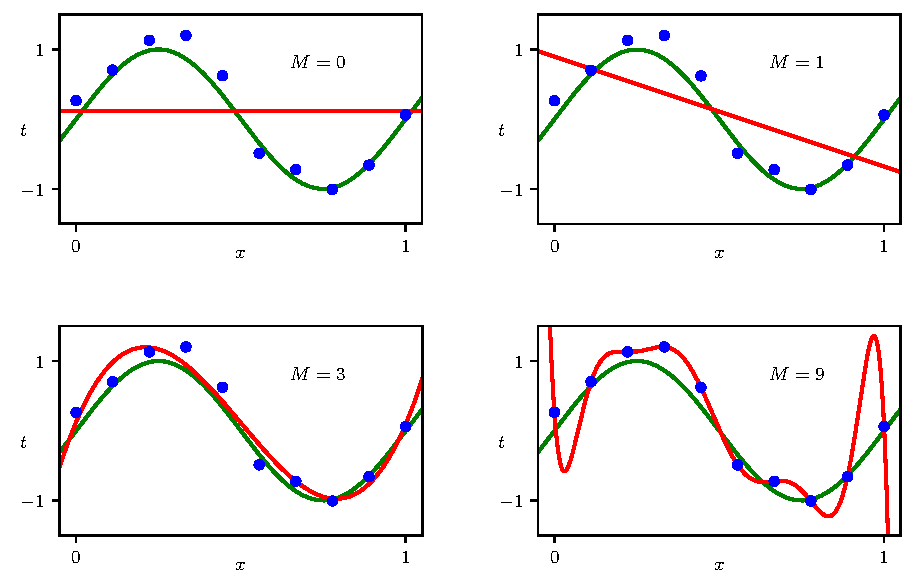
\includegraphics[width=0.88\linewidth]{figures/bishop_polynomial_fits.pdf}
\caption{Polynomial curve fitting with varying degrees of capacity $M \in \{0, 1, 3, 9\}$ on $N = 10$ training samples generated by $t = \sin(2\pi x) + \epsilon$ (blue circles). The green curve represents the true underlying generating function $\sin(2\pi x)$, and the red curve is the least-squares fitted polynomial $y(x, \mathbf{w}) = \sum_{j=0}^M w_j x^j$. For $M = 0$ and $M = 1$, the model underfits (high bias), unable to represent the non-linear sinusoidal pattern. For $M = 3$, the model achieves an optimal balance between capacity and data size. For $M = 9$, the polynomial has 10 free parameters and passes exactly through every training point ($\hat{R}_N = 0$), but exhibits violent oscillations near the boundary domain (Runge's phenomenon), causing catastrophic overfitting (adapted from Bishop~\cite{bishop2024deep}).}
\label{fig:bishop_polynomial_fits}
\end{figure}

The behavior across the four degrees illustrates the capacity spectrum:
\begin{enumerate}[leftmargin=*]
  \item \textbf{Degree $M = 0$ (Constant model):} The hypothesis is a horizontal flat line $y(x) = w_0$, which simply computes the empirical mean of the target values $t_n$. It has zero ability to reflect the spatial variation of $x$, producing massive underfitting.
  \item \textbf{Degree $M = 1$ (Linear model):} The hypothesis is a straight line $y(x) = w_0 + w_1 x$. While it captures the overall negative downward slope across the middle of $[0, 1]$, it is fundamentally incapable of bending to trace the positive and negative lobes of the sine function. High bias dominates.
  \item \textbf{Degree $M = 3$ (Cubic polynomial):} The cubic model possesses sufficient flexibility ($4$ parameters: $w_0, \dots, w_3$) to capture the inflection point and alternating peaks of $\sin(2\pi x)$, while remaining constrained enough to ignore individual noise perturbations. It achieves an optimal trade-off with excellent generalization.
  \item \textbf{Degree $M = 9$ (9th-degree polynomial):} With $M = 9$, the polynomial has $M + 1 = 10$ free parameters $\mathbf{w} = [w_0, \dots, w_9]^\top$, exactly matching the number of data points $N = 10$. The linear system of Normal Equations has a unique exact interpolating solution: the fitted red curve passes \textbf{exactly through every single data point}, yielding $\hat{R}_{\text{train}}(h) = 0$.
  
  However, between the data points—and especially near the boundaries of the interval $[0, 1]$—the curve oscillates wildly, swinging violently into positive and negative extremes. This explosive instability is the classical numerical manifestation known as \textbf{Runge's phenomenon} in high-degree polynomial interpolation. At test time, any point sampled slightly off the training nodes incurs a huge prediction error.
\end{enumerate}

\paragraph{The root mechanical symptom of overfitting: Exploding weight magnitudes.}
Why does the degree-9 polynomial oscillate so violently? When we inspect the numerical values of the optimal weight vector $\mathbf{w}^*$ as $M$ increases, a striking structural pattern emerges:
\begin{itemize}[noitemsep]
  \item For $M = 1$: Weights remain modest: $w_0 \approx 0.8$, $w_1 \approx -1.3$.
  \item For $M = 3$: Weights are comfortably bounded: $w_0 \approx 0.3$, $w_1 \approx 4.9$, $w_2 \approx -10.8$, $w_3 \approx 5.6$.
  \item For $M = 9$: The weights \textbf{explode by multiple orders of magnitude} (reaching magnitudes exceeding $10^5$), alternating between massive positive and negative values.
\end{itemize}
To pass precisely through 10 arbitrarily perturbed points, the high-degree polynomial must execute aggressive, steep turns. A function can only change its slope drastically over minuscule horizontal distances $\Delta x$ if its derivative is enormous, which directly requires astronomical polynomial coefficients $w_j$.

This mathematical realization provides the direct bridge to modern machine learning regularization: if overfitting is mechanically driven by uncontrolled parameter explosion, we can prevent overfitting by penalizing large weight vectors—a technique formalized in Section~\ref{sec:regularization_theory}.

\subsection{Model validation protocols and the Golden Rule of Machine Learning}
\label{sec:validation_protocols}

To detect and prevent overfitting, a machine learner must establish disciplined data splitting protocols.

\paragraph{The Train-Validation-Test partition.}
When a dataset $\mathcal{D}_N$ is provided, it must be partitioned into three strictly isolated subsets:
\begin{equation}
\mathcal{D}_{\text{train}} \quad (60\% - 70\%), \quad \mathcal{D}_{\text{val}} \quad (15\% - 20\%), \quad \mathcal{D}_{\text{test}} \quad (15\% - 20\%).
\end{equation}
\begin{itemize}[noitemsep]
  \item $\mathcal{D}_{\text{train}}$ (Training Set): Used exclusively to fit internal model parameters (e.g., weights $\mathbf{w}$ via gradient descent or least squares).
  \item $\mathcal{D}_{\text{val}}$ (Validation Set): Used to tune \textbf{hyperparameters} (e.g., polynomial degree, learning rate $\eta$, regularization weight $\lambda$) and perform model selection across competing architectures.
  \item $\mathcal{D}_{\text{test}}$ (Test Set): Used exclusively for the final evaluation of generalization performance at deployment time.
\end{itemize}

\paragraph{The Cardinal Rule of Machine Learning.}
In oral examinations, a strict imperative frequently emphasized is the \textbf{Cardinal Rule of Machine Learning}:
\begin{examinsight}[The Cardinal Rule of Machine Learning: Never Touch the Test Set!]
\textbf{Never, EVER use the test set for model selection, hyperparameter tuning, or early stopping!}\\
Using the test set to choose model hyperparameters is statistical cheating. It leaks test information into the training loop, invalidating the i.i.d. assumption and producing severely over-optimistic performance claims that fail when the system is deployed in the real world. The test set must remain locked in a vault, evaluated exactly once at the conclusion of all model design.
\end{examinsight}

\subsection{$k$-Fold and Leave-One-Out cross-validation}
\label{sec:cross_validation}

When the available dataset is small, sequestering a fixed validation set severely reduces the data available for model training. To maximize data efficiency while maintaining rigorous validation, we use \textbf{$k$-Fold Cross-Validation}:
\begin{enumerate}
  \item Partition the training data into $k$ equal-sized disjoint subsets (folds): $\mathcal{D}_1, \mathcal{D}_2, \dots, \mathcal{D}_k$.
  \item Perform $k$ training rounds. In round $i \in \{1, \dots, k\}$:
  \begin{itemize}[noitemsep]
    \item Train the candidate model on the remaining $k-1$ folds: $\bigcup_{j \ne i} \mathcal{D}_j$.
    \item Evaluate empirical validation risk on the held-out fold: $\hat{R}_{\text{val}}^{(i)} = \hat{R}(h; \mathcal{D}_i)$.
  \end{itemize}
  \item Compute the cross-validation performance estimate by averaging across all $k$ rounds:
  \begin{equation}
  \hat{R}_{\text{CV}} = \frac{1}{k} \sum_{i=1}^k \hat{R}_{\text{val}}^{(i)}.
  \label{eq:k_fold_cv_average}
  \end{equation}
\end{enumerate}
Typical choices are $k = 5$ or $k = 10$. 

\paragraph{Leave-One-Out Cross-Validation (LOOCV).}
In the extreme limit where $k = N$ (the total number of training samples):
\begin{itemize}[noitemsep]
  \item Each round trains on $N - 1$ samples and validates on the single remaining sample.
  \item This is repeated $N$ times, averaging errors across all points.
  \item LOOCV provides an almost unbiased estimate of true risk, but is computationally expensive ($O(N)$ full training runs).
\end{itemize}

\subsection{Regularization as a learning solution to overfitting}
\label{sec:regularization_theory}

Cross-validation allows us to select hyperparameters, but how do we prevent a complex model from overfitting directly during optimization? The answer is \textbf{Regularization}: augmenting the empirical risk objective with a penalty that penalizes model complexity.

The regularized empirical risk objective is:
\begin{equation}
\hat{R}_{\text{reg}}(h) \triangleq \hat{R}_N(h) + \lambda \Omega(h) = \frac{1}{N}\sum_{i=1}^N \ell(h(\mathbf{x}_i), y_i) + \lambda \Omega(\mathbf{w}),
\label{eq:regularized_objective}
\end{equation}
where $\Omega(\mathbf{w})$ is a complexity regularizer and $\lambda \ge 0$ is the \textbf{regularization strength} hyperparameter:
\begin{itemize}[noitemsep]
  \item If $\lambda = 0$: Reverts to unconstrained ERM, risking severe overfitting.
  \item If $\lambda \to \infty$: The optimization ignores training data completely, forcing all weights to zero and causing severe underfitting.
  \item Intermediate $\lambda$: Balances empirical fitting fidelity against parameter simplicity.
\end{itemize}

The two canonical forms of regularization in machine learning are:
\begin{enumerate}
  \item \textbf{$L_2$ Regularization (Ridge / Weight Decay)}:
  \begin{equation}
  \Omega(\mathbf{w}) = \frac{1}{2} \|\mathbf{w}\|_2^2 = \frac{1}{2} \sum_{j=1}^d w_j^2.
  \label{eq:l2_regularization}
  \end{equation}
  Drives weight magnitudes smoothly toward zero; prevents any single feature coordinate from exerting disproportionate influence; mathematically equivalent to a zero-mean Gaussian prior.
  \item \textbf{$L_1$ Regularization (Lasso)}:
  \begin{equation}
  \Omega(\mathbf{w}) = \|\mathbf{w}\|_1 = \sum_{j=1}^d |w_j|.
  \label{eq:l1_regularization}
  \end{equation}
  Due to the non-differentiable sharp corners of the $L_1$ ball at coordinate axes, Lasso drives non-essential weights to \textbf{identically zero}, performing automatic feature selection and producing sparse models.
\end{enumerate}

---

\section{Linear predictors, least squares regression, and basis expansion}
\label{sec:linear_predictors_and_least_squares}

\subsection{Linear predictors in 1D and multi-dimensional space}
\label{sec:linear_predictors_formulation}

A \textbf{linear predictor} models the relationship between feature input $\mathbf{x}$ and target $y$ as an affine combination of coordinates:
\begin{itemize}
  \item \textbf{One-Dimensional Predictor}: When the input space is scalar ($\mathcal{X} = \mathbb{R}$), the hypothesis is a straight line:
  \begin{equation}
  \hat{y} = h_{(w,b)}(x) = w x + b,
  \label{eq:linear_predictor_1d}
  \end{equation}
  where $w \in \mathbb{R}$ is the slope weight and $b \in \mathbb{R}$ is the bias offset (y-intercept).
  \item \textbf{Multi-Dimensional Predictor}: When inputs are $d$-dimensional feature vectors ($\mathbf{x} \in \mathbb{R}^d$), the hypothesis is an affine hyperplane:
  \begin{equation}
  \hat{y} = h_{(\mathbf{w},b)}(\mathbf{x}) = \mathbf{w}^\top \mathbf{x} + b = \sum_{j=1}^d w_j x_j + b,
  \label{eq:linear_predictor_multid}
  \end{equation}
  where $\mathbf{w} = [w_1, \dots, w_d]^\top \in \mathbb{R}^d$ is the weight parameter vector.
\end{itemize}

\begin{figure}[htbp]
\centering
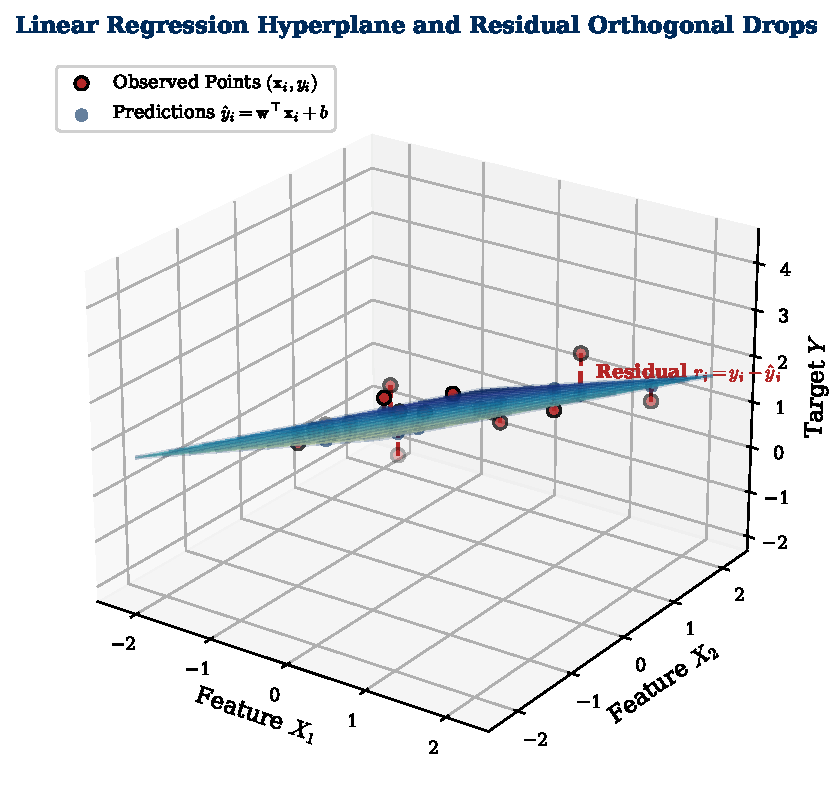
\includegraphics[width=0.72\linewidth]{figures/linear_plane_3d.pdf}
\caption{Geometric representation of a linear predictor for two-dimensional inputs $\mathbf{x} = [x_1, x_2]^\top \in \mathbb{R}^2$ ($h(\mathbf{x}) = w_1 x_1 + w_2 x_2 + b$). In regression, the hypothesis corresponds to a 2D affine hyperplane (colored grid) embedded in 3D feature-target space $(X_1, X_2, Y)$. The observed training instances $(\mathbf{x}_i, y_i)$ are plotted as red spheres, and the vertical drop segments represent the individual residuals $r_i = y_i - \hat{y}_i$ measuring the vertical error between observations and the regression surface.}
\label{fig:linear_plane_3d}
\end{figure}

\paragraph{Geometric interpretation of hyperplanes.}
In classification and regression, the affine equation $\mathbf{w}^\top \mathbf{x} + b = 0$ defines a $(d-1)$-dimensional \textbf{hyperplane}:
\begin{itemize}[noitemsep]
  \item The weight vector $\mathbf{w}$ is the \textbf{orthogonal normal vector} to the hyperplane, pointing toward the positive half-space where $\mathbf{w}^\top \mathbf{x} + b > 0$.
  \item The bias parameter $b$ dictates the orthogonal distance from the coordinate origin to the hyperplane: $\text{distance} = \frac{|b|}{\|\mathbf{w}\|_2}$. If $b = 0$, the hyperplane passes directly through the coordinate origin.
\end{itemize}

\subsection{The Least Squares criterion and matrix-vector formulation}
\label{sec:least_squares_criterion}

For continuous regression, the canonical performance metric is the \textbf{squared loss} $\ell(\hat{y}, y) = \frac{1}{2}(\hat{y} - y)^2$. Under the Empirical Risk Minimization (ERM) framework, the \textbf{Least Squares (LSQ)} criterion searches for the parameter tuple $(\mathbf{w}, b)$ that minimizes the sum (or average) of squared vertical distances between observed training targets $y_i$ and model predictions $\hat{y}_i = h(\mathbf{x}_i)$:
\begin{equation}
J(\mathbf{w}, b) = \frac{1}{2} \sum_{i=1}^N \left( \mathbf{w}^\top \mathbf{x}_i + b - y_i \right)^2.
\label{eq:least_squares_sum_form}
\end{equation}

\paragraph{The geometric meaning of ``Least Squares''.}
\Cref{fig:least_squares_criterion_geometry} illustrates the mechanics of the Least Squares criterion for a 1D linear predictor:
\begin{enumerate}[noitemsep]
  \item For each observed data point $(x_i, y_i)$, the model predicts $\hat{y}_i = wx_i + b$ along the dashed regression line.
  \item The vertical deviation is the \textbf{residual error}:
  \begin{equation}
  r_i \triangleq y_i - \hat{y}_i = y_i - (wx_i + b).
  \label{eq:residual_error_def}
  \end{equation}
  \item The squared loss $\ell_i = r_i^2$ corresponds literally to the \textbf{area of a geometric square} with side length $|r_i|$. The name \emph{Least Squares} originates from the objective of finding the line orientation that minimizes the total aggregate area of all shaded squares.
  \item Once the optimal parameters $(w^*, b^*)$ are learned, the model serves as an inference engine: given any new, unseen query feature $x_0$, the predictor projects $x_0$ vertically onto the fitted line to output the predicted target $\hat{y}_0 = w^* x_0 + b^*$.
\end{enumerate}

\begin{figure}[htbp]
\centering
\begin{tikzpicture}[scale=1.05]
  % Axes
  \draw[-{Stealth[length=2.5mm]}, thick] (0, 0) -- (11.0, 0) node[below=1.5mm, font=\small\sffamily] {Feature input $x$};
  \draw[-{Stealth[length=2.5mm]}, thick] (0, 0) -- (0, 6.6) node[left=1.5mm, font=\small\sffamily] {Target output $y$};
  
  % Bias intercept on y-axis
  \draw[thick] (-0.1, 1.2) -- (0.1, 1.2) node[left=2mm, font=\small\bfseries\sffamily, text=politoNavy] {Intercept $b$};
  
  % Regression line: y = 0.55*x + 1.2
  \draw[very thick, dashed, examred] (0.2, 1.31) -- (9.8, 6.59) 
    node[pos=0.96, above left=1mm, font=\small\bfseries\sffamily, text=examred] {$\hat{y} = wx + b$};

  % Geometric square areas for residuals (r_i^2)
  % Point 1: x=1.6, y=1.4, yhat=2.08, r=-0.68
  \fill[deepblue!15, draw=deepblue!60, thin] (1.6, 1.4) rectangle (1.6 + 0.68, 2.08);
  % Point 2: x=2.8, y=3.7, yhat=2.74, r=+0.96
  \fill[deepblue!15, draw=deepblue!60, thin] (2.8, 2.74) rectangle (2.8 + 0.96, 3.7);
  % Point 3: x=4.3, y=2.9, yhat=3.565, r=-0.665
  \fill[deepblue!15, draw=deepblue!60, thin] (4.3, 2.9) rectangle (4.3 + 0.665, 3.565);
  % Point 4: x=7.0, y=5.8, yhat=5.05, r=+0.75
  \fill[deepblue!15, draw=deepblue!60, thin] (7.0, 5.05) rectangle (7.0 + 0.75, 5.8);
  % Point 5: x=8.3, y=5.1, yhat=5.765, r=-0.665
  \fill[deepblue!15, draw=deepblue!60, thin] (8.3, 5.1) rectangle (8.3 + 0.665, 5.765);

  % Residual vertical lines
  \draw[thick, deepblue] (1.6, 1.4) -- (1.6, 2.08);
  \draw[thick, deepblue] (2.8, 3.7) -- (2.8, 2.74);
  \draw[thick, deepblue] (4.3, 2.9) -- (4.3, 3.565);
  \draw[thick, deepblue] (7.0, 5.8) -- (7.0, 5.05);
  \draw[thick, deepblue] (8.3, 5.1) -- (8.3, 5.765);

  % Fitted predictions (red dots on the line)
  \foreach \coord in {(1.6, 2.08), (2.8, 2.74), (4.3, 3.565), (7.0, 5.05), (8.3, 5.765)} {
    \fill[examred] \coord circle (1.8pt);
  }

  % Training points (xi, yi) (blue dots)
  \foreach \coord in {(1.6, 1.4), (2.8, 3.7), (4.3, 2.9), (7.0, 5.8), (8.3, 5.1)} {
    \fill[politoNavy] \coord circle (2.8pt);
    \draw[black, thick] \coord circle (2.8pt);
  }

  % Annotation for Training sample (pointing to Point 2)
  \draw[-{Stealth[length=1.5mm]}, thick, politoNavy] (1.8, 4.7) node[above, font=\footnotesize\bfseries\sffamily, text=politoNavy] {Training sample $(x_i, y_i)$} -- (2.7, 3.8);

  % Annotation for Residual and Squared Loss (pointing to Point 4)
  \draw[-{Stealth[length=1.5mm]}, thick, deepblue] (8.5, 5.4) -- (7.8, 5.4) 
    node[pos=0, right=1mm, font=\scriptsize\sffamily, align=left, text=deepblue] {
      \textbf{Vertical residual:}\\
      $r_i = y_i - \hat{y}_i = y_i - (wx_i + b)$\\[0.5ex]
      \textbf{Squared loss area:}\\
      $\ell_i = (y_i - \hat{y}_i)^2 = r_i^2$
    };

  % Query prediction x0
  \draw[thick, dashed, deepdiveTeal] (5.6, 0) -- (5.6, 4.28) -- (0, 4.28);
  \fill[deepdiveTeal] (5.6, 4.28) circle (2.8pt);
  \draw[black, thick] (5.6, 4.28) circle (2.8pt);
  \draw[thick] (5.6, 0.1) -- (5.6, -0.1) node[below=1mm, font=\small\bfseries\sffamily, text=deepdiveTeal] {Query $x_0$};
  \draw[thick] (0.1, 4.28) -- (-0.1, 4.28) node[left=1mm, font=\small\bfseries\sffamily, text=deepdiveTeal] {$\hat{y}_0 = h(x_0)$};
  \node[anchor=south east, font=\scriptsize\bfseries\sffamily, text=deepdiveTeal] at (5.55, 4.35) {Prediction $\hat{y}_0 = wx_0 + b$};

  % Summary formula callout
  \node[rectangle, draw=black!70, fill=white, rounded corners=1mm, font=\footnotesize\sffamily, align=center] at (6.5, 1.5) {
    \textbf{\color{politoNavy}Least Squares (LSQ) Fitting Criterion}:\\[0.5ex]
    $h_{\text{LSQ}} = \argmin_{w, b} \dfrac{1}{N} \sum_{i=1}^N \underbrace{\left( y_i - (w x_i + b) \right)^2}_{\text{Sum of squared residual areas } r_i^2}$
  };
\end{tikzpicture}
\caption{The geometry of linear predictors and the Least Squares (LSQ) criterion in one dimension. The hypothesis $\hat{y} = wx + b$ seeks parameters $(w, b)$ that minimize the aggregate sum of squared vertical residuals (represented by the shaded square areas $r_i^2$). For any new query input $x_0$, the model outputs prediction $\hat{y}_0 = h(x_0) = wx_0 + b$ via vertical projection onto the fitted regression line.}
\label{fig:least_squares_criterion_geometry}
\end{figure}

\paragraph{The bias absorption trick.}
To streamline matrix calculus, we absorb the scalar bias $b$ into the weight vector by augmenting each feature vector with a dummy constant coordinate of 1:
\begin{equation}
\mathbf{x}' \triangleq \begin{bmatrix} 1 \\ \mathbf{x} \end{bmatrix} = \begin{bmatrix} 1 \\ x_1 \\ \vdots \\ x_d \end{bmatrix} \in \mathbb{R}^{d+1}, \quad \mathbf{w}' \triangleq \begin{bmatrix} b \\ \mathbf{w} \end{bmatrix} = \begin{bmatrix} b \\ w_1 \\ \vdots \\ w_d \end{bmatrix} \in \mathbb{R}^{d+1}.
\label{eq:bias_absorption_trick}
\end{equation}
Under this homogeneous notation, $\mathbf{w}'^\top \mathbf{x}' = b \cdot 1 + \mathbf{w}^\top \mathbf{x} = \mathbf{w}^\top \mathbf{x} + b$. For the remainder of this derivation, we assume $\mathbf{X}$ and $\mathbf{w}$ represent the augmented coordinates.

We construct the \textbf{Design Matrix} $\mathbf{X} \in \mathbb{R}^{N \times (d+1)}$ by stacking all $N$ augmented sample vectors as rows, and the target vector $\mathbf{y} \in \mathbb{R}^N$:
\begin{equation}
\mathbf{X} = \begin{bmatrix} \mathbf{x}_1^\top \\ \mathbf{x}_2^\top \\ \vdots \\ \mathbf{x}_N^\top \end{bmatrix} = \begin{bmatrix} 1 & x_{11} & \dots & x_{1d} \\ 1 & x_{21} & \dots & x_{2d} \\ \vdots & \vdots & \ddots & \vdots \\ 1 & x_{N1} & \dots & x_{Nd} \end{bmatrix}, \quad \mathbf{y} = \begin{bmatrix} y_1 \\ y_2 \\ \vdots \\ y_N \end{bmatrix}.
\label{eq:design_matrix_form}
\end{equation}
The vector of model predictions across all $N$ training samples is simply the matrix-vector product $\hat{\mathbf{y}} = \mathbf{X}\mathbf{w} \in \mathbb{R}^N$. The empirical loss in compact matrix notation becomes:
\begin{equation}
J(\mathbf{w}) = \frac{1}{2} \|\mathbf{X}\mathbf{w} - \mathbf{y}\|_2^2 = \frac{1}{2} (\mathbf{X}\mathbf{w} - \mathbf{y})^\top (\mathbf{X}\mathbf{w} - \mathbf{y}).
\label{eq:least_squares_matrix_objective}
\end{equation}

\subsection{Analytical derivation of the Normal Equations via matrix calculus}
\label{sec:normal_equations_derivation}

Because $J(\mathbf{w})$ is a convex quadratic function of $\mathbf{w}$, its global minimum occurs where the gradient vector with respect to $\mathbf{w}$ vanishes: $\nabla_{\mathbf{w}} J(\mathbf{w}) = \mathbf{0}$.

\begin{proof}[Analytical Derivation of the Normal Equations]
Expanding the quadratic form in Equation~\eqref{eq:least_squares_matrix_objective}:
\begin{align}
J(\mathbf{w}) &= \frac{1}{2} \left( (\mathbf{X}\mathbf{w})^\top - \mathbf{y}^\top \right) (\mathbf{X}\mathbf{w} - \mathbf{y}) \nonumber \\
&= \frac{1}{2} \left( \mathbf{w}^\top \mathbf{X}^\top \mathbf{X} \mathbf{w} - \mathbf{w}^\top \mathbf{X}^\top \mathbf{y} - \mathbf{y}^\top \mathbf{X} \mathbf{w} + \mathbf{y}^\top \mathbf{y} \right).
\end{align}
Because $\mathbf{w}^\top \mathbf{X}^\top \mathbf{y}$ is a scalar, it equals its own transpose: $\mathbf{w}^\top \mathbf{X}^\top \mathbf{y} = (\mathbf{w}^\top \mathbf{X}^\top \mathbf{y})^\top = \mathbf{y}^\top \mathbf{X} \mathbf{w}$. Combining the cross-terms:
\begin{equation}
J(\mathbf{w}) = \frac{1}{2} \mathbf{w}^\top (\mathbf{X}^\top \mathbf{X}) \mathbf{w} - \mathbf{w}^\top (\mathbf{X}^\top \mathbf{y}) + \frac{1}{2} \mathbf{y}^\top \mathbf{y}.
\label{eq:expanded_matrix_loss}
\end{equation}

Now, compute the vector derivative $\nabla_{\mathbf{w}} J(\mathbf{w})$ using standard matrix calculus identities ($\nabla_{\mathbf{w}} (\mathbf{w}^\top \mathbf{A} \mathbf{w}) = (\mathbf{A} + \mathbf{A}^\top)\mathbf{w} = 2\mathbf{A}\mathbf{w}$ for symmetric $\mathbf{A} = \mathbf{X}^\top \mathbf{X}$, and $\nabla_{\mathbf{w}} (\mathbf{w}^\top \mathbf{b}) = \mathbf{b}$):
\begin{equation}
\nabla_{\mathbf{w}} J(\mathbf{w}) = \mathbf{X}^\top \mathbf{X} \mathbf{w} - \mathbf{X}^\top \mathbf{y}.
\label{eq:least_squares_gradient}
\end{equation}
Setting the gradient identically to zero:
\begin{equation}
\mathbf{X}^\top \mathbf{X} \mathbf{w} - \mathbf{X}^\top \mathbf{y} = \mathbf{0}.
\end{equation}
This yields the celebrated \textbf{Normal Equations}:
\begin{equation}
\mathbf{X}^\top \mathbf{X} \mathbf{w} = \mathbf{X}^\top \mathbf{y}.
\label{eq:normal_equations}
\end{equation}
Assuming the square matrix $\mathbf{X}^\top \mathbf{X} \in \mathbb{R}^{(d+1) \times (d+1)}$ is invertible (full column rank), multiplying both sides by $(\mathbf{X}^\top \mathbf{X})^{-1}$ gives the unique closed-form \textbf{Ordinary Least Squares (OLS)} estimator:
\begin{equation}
\mathbf{w}^* = (\mathbf{X}^\top \mathbf{X})^{-1} \mathbf{X}^\top \mathbf{y}.
\label{eq:ols_closed_form}
\end{equation}
\end{proof}

\subsection{Regularized Least Squares: Closed-form Ridge Regression}
\label{sec:ridge_regression_derivation}

What happens if $\mathbf{X}^\top \mathbf{X}$ is not invertible? This failure occurs when:
\begin{itemize}[noitemsep]
  \item Features are collinear (redundant columns in $\mathbf{X}$).
  \item The number of features exceeds the number of training samples ($d > N$).
\end{itemize}
To guarantee invertibility and prevent overfitting, we add $L_2$ regularization:
\begin{equation}
J_{\text{ridge}}(\mathbf{w}) = \frac{1}{2} \|\mathbf{X}\mathbf{w} - \mathbf{y}\|_2^2 + \frac{\lambda}{2} \|\mathbf{w}\|_2^2, \quad \lambda > 0.
\label{eq:ridge_objective}
\end{equation}

Computing the gradient of the regularized objective:
\begin{equation}
\nabla_{\mathbf{w}} J_{\text{ridge}}(\mathbf{w}) = \mathbf{X}^\top \mathbf{X} \mathbf{w} - \mathbf{X}^\top \mathbf{y} + \lambda \mathbf{w} = (\mathbf{X}^\top \mathbf{X} + \lambda \mathbf{I}) \mathbf{w} - \mathbf{X}^\top \mathbf{y}.
\end{equation}
Setting the gradient to zero:
\begin{equation}
(\mathbf{X}^\top \mathbf{X} + \lambda \mathbf{I}) \mathbf{w} = \mathbf{X}^\top \mathbf{y}.
\label{eq:ridge_normal_equations}
\end{equation}
Multiplying by the inverse yields the closed-form \textbf{Ridge Regression} solution:
\begin{equation}
\mathbf{w}^*_{\text{ridge}} = (\mathbf{X}^\top \mathbf{X} + \lambda \mathbf{I})^{-1} \mathbf{X}^\top \mathbf{y}.
\label{eq:ridge_closed_form}
\end{equation}

\paragraph{Mathematical guarantee of invertibility.}
Why is $(\mathbf{X}^\top \mathbf{X} + \lambda \mathbf{I})$ guaranteed to be invertible for any $\lambda > 0$?
\begin{itemize}[noitemsep]
  \item The matrix $\mathbf{X}^\top \mathbf{X}$ is symmetric and positive semi-definite: all its eigenvalues satisfy $\mu_i \ge 0$.
  \item Adding $\lambda \mathbf{I}$ shifts every eigenvalue strictly by $\lambda$:
  \begin{equation}
  \operatorname{eig}_i(\mathbf{X}^\top \mathbf{X} + \lambda \mathbf{I}) = \mu_i + \lambda \ge \lambda > 0.
  \end{equation}
  \item Because all eigenvalues are strictly positive ($\lambda > 0$), the determinant $\det(\mathbf{X}^\top \mathbf{X} + \lambda \mathbf{I}) = \prod_i (\mu_i + \lambda) > 0$. The matrix is strictly \textbf{positive definite and guaranteed invertible}, stabilizing matrix conditioning even in high-dimensional $d \gg N$ regimes.
\end{itemize}

\subsection{Beyond linear models: Non-linear fitting via polynomial basis expansion}
\label{sec:basis_expansion}

Linear regression appears restricted to planar surfaces. Can we use linear regression to fit arbitrary non-linear curves?

The answer is yes, through the technique of \textbf{Basis Function Expansion}. Instead of operating directly on the raw input scalar $x \in \mathbb{R}$, we map $x$ into a high-dimensional feature space using fixed non-linear basis transformations:
\begin{equation}
\boldsymbol{\phi}(x) = [1, \phi_1(x), \phi_2(x), \dots, \phi_p(x)]^\top \in \mathbb{R}^{p+1}.
\label{eq:basis_expansion_mapping}
\end{equation}
For polynomial regression of degree $p$:
\begin{equation}
\boldsymbol{\phi}(x) = [1, x, x^2, x^3, \dots, x^p]^\top.
\label{eq:polynomial_basis_vector}
\end{equation}
The prediction model becomes:
\begin{equation}
h(x) = \mathbf{w}^\top \boldsymbol{\phi}(x) = w_0 + w_1 x + w_2 x^2 + \dots + w_p x^p.
\label{eq:polynomial_linear_in_parameters}
\end{equation}

Crucially, \textbf{$h(x)$ is non-linear with respect to the input $x$, but strictly linear with respect to the parameters $\mathbf{w}$!} 

Therefore, we can construct the feature matrix $\mathbf{\Phi} \in \mathbb{R}^{N \times (p+1)}$ where row $i$ is $\boldsymbol{\phi}(x_i)^\top$, and solve for the optimal weights using the exact same closed-form Normal Equations derived in Equation~\eqref{eq:ols_closed_form}:
\begin{equation}
\mathbf{w}^* = (\mathbf{\Phi}^\top \mathbf{\Phi})^{-1} \mathbf{\Phi}^\top \mathbf{y}.
\label{eq:basis_normal_equations}
\end{equation}

\paragraph{The conceptual bridge to Chapter~\ref{sec:optimization_and_gradient_descent}: The dual motivation for Gradient Descent.}
The closed-form Normal Equations $\mathbf{w}^* = (\mathbf{X}^\top \mathbf{X})^{-1}\mathbf{X}^\top \mathbf{y}$ (and its regularized counterpart in Equation~\eqref{eq:ridge_closed_form}) represent an elegant analytical result. However, students must recognize that the existence of this closed-form solution is a \textbf{rare, fortunate mathematical coincidence} rather than the general norm in machine learning. 

Analytically reducing the stationary condition $\nabla_{\mathbf{w}} J(\mathbf{w}) = \mathbf{0}$ to a linear matrix equation solvable via direct matrix inversion ($\mathbf{A}\mathbf{w} = \mathbf{b} \implies \mathbf{w}^* = \mathbf{A}^{-1}\mathbf{b}$) holds as an exact equivalence ($\iff$) if and only if two conditions coincide simultaneously:
\begin{enumerate}[noitemsep]
  \item The predictor $h(\mathbf{x})$ is strictly \textbf{linear in its parameter vector} $\mathbf{w}$ (as in linear regression or fixed basis expansions).
  \item The loss function $\ell(\hat{y}, y)$ is strictly \textbf{quadratic in its prediction} $\hat{y}$ (such as standard squared error, weighted least squares, or ridge regularizers).
\end{enumerate}
Only under this exact pairing does the empirical objective $J(\mathbf{w})$ form a purely quadratic polynomial in $\mathbf{w}$, ensuring that its gradient $\nabla_{\mathbf{w}} J(\mathbf{w}) = \mathbf{A}\mathbf{w} - \mathbf{b}$ is strictly \emph{affine} (linear in $\mathbf{w}$), which yields a linear algebraic system of equations solvable by matrix inversion. (Note that for the existence of closed-form solutions in general, this condition is only sufficient ($\impliedby$) but not necessary, as analytical closed forms also arise in generative models like Naive Bayes or median estimation under $L_1$ loss; however, for solvability specifically via \emph{linear matrix inversion}, it is an exact $\iff$ equivalence).

In modern machine learning, this algebraic convenience collapses across two fundamental dimensions, establishing the \textbf{dual motivation} for first-order numerical optimization:
\begin{itemize}
  \item \textbf{1. Mathematical Necessity (Non-solvability for General and Non-Convex Losses):} 
  The moment we step outside quadratic loss, setting the gradient to zero no longer yields a linear system:
  \begin{itemize}[noitemsep]
    \item \emph{Convex, non-quadratic losses:} Even for elementary linear models, if we adopt Cross-Entropy (Logistic Loss) for classification, setting $\nabla_{\mathbf{w}} J(\mathbf{w}) = \sum_{i=1}^N (\sigma(\mathbf{w}^\top \mathbf{x}_i) - y_i)\mathbf{x}_i = \mathbf{0}$ produces a coupled system of \textbf{transcendental, non-linear equations}. No algebraic matrix inversion can ever isolate $\mathbf{w}^*$, despite the objective being strictly convex. The same analytical impossibility applies to Hinge loss (SVMs) and $L_1$ loss.
    \item \emph{Non-convex landscapes and Neural Networks:} When models introduce non-linear parameter compositions (as in deep neural networks $h_{\mathbf{w}}(\mathbf{x}) = \mathbf{W}_L \sigma(\mathbf{W}_{L-1} \dots \sigma(\mathbf{W}_1 \mathbf{x}))$), the empirical loss surface $J(\mathbf{w})$ becomes highly non-convex, populated by intricate configurations of local minima, ravines, and saddle points. Here, algebraic inversion is conceptually and mathematically impossible. An iterative algorithm is the \emph{sole viable mechanism} to navigate the landscape.
  \end{itemize}
  
  \item \textbf{2. Computational Intractability (High-Dimensional Scaling):}
  Even in the ideal textbook scenario where a closed-form solution exists (linear model with MSE), evaluating $(\mathbf{X}^\top \mathbf{X})^{-1}\mathbf{X}^\top \mathbf{y}$ is computationally prohibitive for high-dimensional problems:
  \begin{itemize}[noitemsep]
    \item Computing the Gram matrix $\mathbf{X}^\top \mathbf{X}$ requires $\mathcal{O}(N d^2)$ floating-point operations.
    \item Inverting the $(d \times d)$ matrix requires Gaussian elimination or Cholesky factorization scaling cubically as $\mathcal{O}(d^3)$, and demands $\mathcal{O}(d^2)$ memory to store.
    \item When feature representations or neural architectures contain millions or billions of parameters ($d \ge 10^6$), materializing and inverting a $(d \times d)$ matrix exceeds the physical memory and compute capacity of modern computing clusters.
  \end{itemize}
\end{itemize}

Therefore, whether driven by \textbf{mathematical necessity} (non-convex, non-linear, and transcendental loss objectives where closed forms do not exist) or by \textbf{computational necessity} (high-dimensional regimes where matrix inversion is computationally intractable), machine learning must abandon closed-form algebraic solutions. Instead, we must embrace iterative, first-order local optimization: \textbf{Gradient Descent}. 

How to navigate non-linear loss surfaces, escape saddle points, and optimize non-convex objectives iteratively forms the foundational core of Chapter~\ref{sec:optimization_and_gradient_descent}.
